% removed_slides.tex - NOT compiled. Frames taken out of ALIGNN_PINK_presentation.tex
% in the 2026-10-06 'cut and clean' (branch deck-cleanup). Original deck = commit b5fb667
% (62 pages). Old page numbers refer to that PDF. To restore a frame, copy it back between
% \begin{document} and \end{document}; it uses the same theme.tex / metrics.tex macros.
% Some numbers in these frames were later found wrong - see presentation/refine/
% step3_number_changelog.csv before reusing any of them.

% =============================================================================
%  PART A - frames removed outright
% =============================================================================

% -----------------------------------------------------------------------------
% OLD PAGE 2: Where the project stands
% why removed: part divider
% -----------------------------------------------------------------------------
\PartSlide{ONE}{Where the project stands}{PINK reproduced, then extended --- and what the extension is for}

% -----------------------------------------------------------------------------
% OLD PAGE 6: ALIGNN: from CIF to two graphs
% why removed: part divider
% -----------------------------------------------------------------------------
\PartSlide{TWO}{ALIGNN: from CIF to two graphs}{The one structural idea that separates it from CGCNN}

% -----------------------------------------------------------------------------
% OLD PAGE 14: One crystal through CGCNN
% why removed: CGCNN layer-by-layer (facts -> new 10)
% -----------------------------------------------------------------------------
\begin{frame}
\SlideHeader{08b \textperiodcentered\ IMPLEMENTATION}{One crystal through CGCNN}

\begin{center}
{\sffamily\scriptsize
\begin{tabular}{@{}llrr@{}}
\toprule
\textbf{stage} & \textbf{what happens} & \textbf{shape out} & \textbf{weights} \\
\midrule
input   & each atom: a fixed 92-number element fingerprint (group, radius, \ldots)
        & $N \times 92$ & --- \\
        & each bond: its length spread over 41 Gaussians, 0--8 \AA\ in 0.2 \AA\ steps
        & $N \times 12 \times 41$ & --- \\
embed   & one linear layer, 92 $\rightarrow$ 64 & $N \times 64$ & 5{,}952 \\
conv $\times$3 & per neighbour: [self 64 $\Vert$ neighbour 64 $\Vert$ bond 41] = 169 $\rightarrow$ 128,
          & & \\
        & \quad halves: a \emph{gate} (sigmoid, 0--1) $\times$ a \emph{message} (softplus);
          & & \\
        & \quad sum the 12 gated messages, add to the atom's own vector
          & $N \times 64$ & 3 $\times$ 22{,}144 \\
pool    & average over the $N$ atoms of the cell --- size-independent
        & $1 \times 64$ & --- \\
widen   & softplus, linear 64 $\rightarrow$ 128, softplus = \textbf{the hidden features}
        & $1 \times 128$ & 8{,}320 \\
output  & a weighted sum of those 128 numbers + a bias = $\log_{10} K$ (scaled)
        & 1 & 129 \\
\midrule
\textbf{total} & & & \textbf{80{,}833} \\
\bottomrule
\end{tabular}}
\end{center}

\vspace{2pt}
{\sffamily\scriptsize
$N$ = atoms in the cell. The gate is the CGCNN idea: the network learns, per
neighbour, \emph{how much} to listen (gate) separately from \emph{what} it hears
(message). Three rounds of this let information travel three bonds.\par}

\Takeaway{ALIGNN keeps the same skeleton --- embed, message-pass, average, one
number out --- but runs it on two graphs (atoms and bonds-with-angles), 4 + 4
layers, 256 wide: $\approx$4.0 million weights, about 50$\times$ CGCNN.}
\end{frame}

% -----------------------------------------------------------------------------
% OLD PAGE 15: Training settings, from the saved runs
% why removed: training settings (facts -> new 10)
% -----------------------------------------------------------------------------
\begin{frame}
\SlideHeader{08c \textperiodcentered\ IMPLEMENTATION}{Training settings, from the saved runs}

\begin{columns}[T]
\column{0.60\linewidth}
{\sffamily\scriptsize
\begin{tabular}{@{}lll@{}}
\toprule
& \textbf{CGCNN} & \textbf{ALIGNN} \\
\midrule
read from        & checkpoint \texttt{.pth}      & \texttt{config.json} per run \\
target           & $\log_{10} K$ or $\log_{10} G$ & same, one model each \\
split            & 7{,}691 / 1{,}648 / 1{,}648   & same crystal ids \\
neighbours       & 12 nearest within 8 \AA       & 12 nearest, 5 \AA\ cutoff \\
bond input       & 41 Gaussians                  & 80 (lengths) + 40 (angles) \\
width            & atoms 64, head 128            & embed 64, hidden 256 \\
layers           & 3 graph convolutions          & 4 ALIGNN + 4 GCN \\
weights          & 80{,}833                      & $\approx$4.0 M \\
loss             & mean squared error            & mean squared error \\
optimiser        & Adam, lr 0.01                 & AdamW, lr 0.001 \\
weight decay     & $10^{-5}$                     & $10^{-5}$ \\
schedule         & cosine                        & one-cycle \\
batch / epochs   & 128 / 200                     & 64 / 150 \\
seeds            & 42, 1, 2                      & 123; then 42, 1, 2 \\
\bottomrule
\end{tabular}}

\column{0.36\linewidth}
\AccentCard{4.6cm}{SlideBlue}{%
  \sffamily\scriptsize
  \textbf{Why $\log_{10}$, not GPa}\\[2pt]
  Moduli span more than two orders of magnitude. In log space a 10\% miss costs
  the same on soft and stiff crystals --- and the screen lives among the soft
  ones.\par}

\vspace{4pt}
\AccentCard{4.6cm}{SlideGreen}{%
  \sffamily\scriptsize
  \textbf{Why two models, not one}\\[2pt]
  $K$ and $G$ each get their own network. The probe on 12c shows why: the $K$
  network carries $G$ only as far as $K$ itself does.\par}

\vspace{4pt}
\AccentCard{4.6cm}{SlideAmber}{%
  \sffamily\scriptsize
  \textbf{Not identical recipes}\\[2pt]
  Split, targets, loss and decay match; optimiser, rate, schedule, batch and
  epochs are each model's own default. The gap is architecture \emph{plus}
  recipe.\par}
\end{columns}
\end{frame}

% -----------------------------------------------------------------------------
% OLD PAGE 16: Training and accuracy
% why removed: part divider
% -----------------------------------------------------------------------------
\PartSlide{THREE}{Training and accuracy}{The dataset, the fit, and where it fails}

% -----------------------------------------------------------------------------
% OLD PAGE 21: The hidden features of CGCNN
% why removed: CGCNN hidden features
% -----------------------------------------------------------------------------
\begin{frame}
\SlideHeader{12b \textperiodcentered\ INSIDE THE MODEL}{The hidden features of CGCNN}

\begin{columns}[T]
\column{0.52\linewidth}
{\sffamily\footnotesize
The last layer of CGCNN (slide 08b) is only a weighted sum:
\[
\log_{10} K \;=\; w_1 h_1 + w_2 h_2 + \dots + w_{128} h_{128} + b
\]
The 128 numbers $h$ are the \textbf{hidden features} --- everything the network
knows about a crystal when it predicts.

\vspace{4pt}
\textbf{How they were read:} a ``hook'' copies $h$ as each of the 1{,}648
\emph{test} crystals passes through the trained $K$ model (seed 42). Nothing is
retrained.

\vspace{4pt}
\textbf{How they are drawn:} PCA rotates the 128-dimensional cloud so axis 1
follows its largest spread, axis 2 the next; the map plots those two.\par}

\column{0.44\linewidth}
\AccentCard{5.3cm}{SlideGreen}{%
  \sffamily\scriptsize
  \textbf{Checked first}\\[2pt]
  This run's predictions equal the saved ones to $2.4\times10^{-7}$ in
  $\log_{10}$ --- the right model, crystals and graphs were loaded.\par}

\vspace{5pt}
\Card{5.3cm}{CardBg}{CardRule}{%
  \sffamily\scriptsize
  \textbf{128 numbers, effectively two}\\[3pt]
  \begin{tabular}{@{}lr@{}}
  share of the spread on PC1 & 76.6\% \\
  on PC2                     & 22.4\% \\
  on PC3                     & 0.85\% \\
  \midrule
  correlation of PC1 with true $\log_{10} K$ & $+0.91$ \\
  \end{tabular}}
\end{columns}

\Takeaway{Before answering, the network squeezes a crystal to about two numbers.
The first is, in effect, ``how stiff''; slide 12c shows what the second separates.}
\end{frame}

% -----------------------------------------------------------------------------
% OLD PAGE 22: The hidden-feature map of 1,648 crystals
% why removed: PCA map
% -----------------------------------------------------------------------------
\begin{frame}
\SlideHeader{12c \textperiodcentered\ INSIDE THE MODEL}{The hidden-feature map of 1{,}648 crystals}

\begin{center}
\includegraphics[width=0.90\linewidth]{figures/hidden_features.png}
\end{center}

\vspace{-8pt}
\begin{columns}[T]
\column{0.31\linewidth}
{\sffamily\scriptsize
\textbf{A.} Soft (dark) to stiff (yellow) runs along PC1. The map is a
\textbf{V}: two arms meeting at a tip.\par}
\column{0.33\linewidth}
{\sffamily\scriptsize
\textbf{B.} Left arm 611 crystals (median $K$ 41 GPa), right arm 1{,}037
(129 GPa). The \textbf{72 off the arms} have 3$\times$ the error (median 0.099 vs
0.034 $\log_{10}$); 40 are oxides. \textcolor{Muted}{Off-arm cut 1.0: set by eye,
not tuned.}\par}
\column{0.31\linewidth}
{\sffamily\scriptsize
\textbf{C.} A straight-line probe reads $G$ from the 128 features at
$R^2 = 0.785$ --- but predicted $K$ alone gives 0.758. Only +0.026 is new; a
real $G$ model reaches 0.889.\par}
\end{columns}

\Takeaway{Where a crystal lands on this map flags where the model is unsure.
And the $K$ network knows $G$ only through $K$ --- the reason $G$ gets its own
network.}
\end{frame}

% -----------------------------------------------------------------------------
% OLD PAGE 24: The physics
% why removed: part divider
% -----------------------------------------------------------------------------
\PartSlide{FOUR}{The physics}{From two moduli to a thermal conductivity}

% -----------------------------------------------------------------------------
% OLD PAGE 30: Validation against measurement
% why removed: part divider
% -----------------------------------------------------------------------------
\PartSlide{FIVE}{Validation against measurement}{45 materials where the answer is known}

% -----------------------------------------------------------------------------
% OLD PAGE 33: The comparison sheet
% why removed: comparison sheet (rows -> new 18)
% -----------------------------------------------------------------------------
\begin{frame}
\SlideHeader{18 \textperiodcentered\ REAL DATA}{The comparison sheet}

\begin{center}
{\sffamily\scriptsize
\begin{tabular}{@{}lrrrr@{}}
\toprule
material & measured & ours (derived $\gamma$) & ours (equal footing) & PINK \\
\midrule
AgCl    &    1.0 &    0.23 &    0.71 &    1.09 \\
Bi$_2$Te$_3$ & 1.6 & 1.24 &   1.43 &    1.20 \\
NaI     &    1.8 &    1.00 &    1.66 &    1.52 \\
PbTe    &    2.5 &    5.72 &    3.74 &    2.71 \\
\midrule
\multicolumn{5}{@{}l@{}}{\color{Muted}\dots\ 37 more \dots} \\
\midrule
AlN     &  350.0 &   55.87 &  118.49 &  140.93 \\
SiC     &  490.0 &  251.19 &  360.10 &  438.31 \\
BN      &  760.0 &  779.67 &  913.63 &  727.98 \\
C (diamond) & 3000.0 & 1180.18 & 1260.63 & 1320.87 \\
\bottomrule
\end{tabular}}
\end{center}

\vspace{3pt}
{\sffamily\footnotesize
\texttt{results/cgcnn/63\_experimental\_vs\_predicted.csv} --- 45 rows,
27 columns. Both $\gamma$ conventions are carried per material, along with each
model's moduli, all three $\gamma$ values, and the p05/p95 interval, so the
choice is visible rather than baked in.}

\Takeaway{ALIGNN is \emph{worse} here --- 0.450 against the CGCNN ensemble's
0.427. It wins on matbench moduli and loses on measured $\kappa_L$. That was
tested, not assumed.}
\end{frame}

% -----------------------------------------------------------------------------
% OLD PAGE 35: The screen
% why removed: part divider
% -----------------------------------------------------------------------------
\PartSlide{SIX}{The screen}{554{,}054 materials, scored twice}

% -----------------------------------------------------------------------------
% OLD PAGE 38: ALIGNN over the whole screen, for the first time
% why removed: ALIGNN vs round 9 (rebuilt as new 23)
% -----------------------------------------------------------------------------
\begin{frame}
\SlideHeader{22 \textperiodcentered\ THE SCREEN}{ALIGNN over the whole screen, for the first time}

\begin{columns}[T]
\column{0.52\linewidth}
\begin{center}
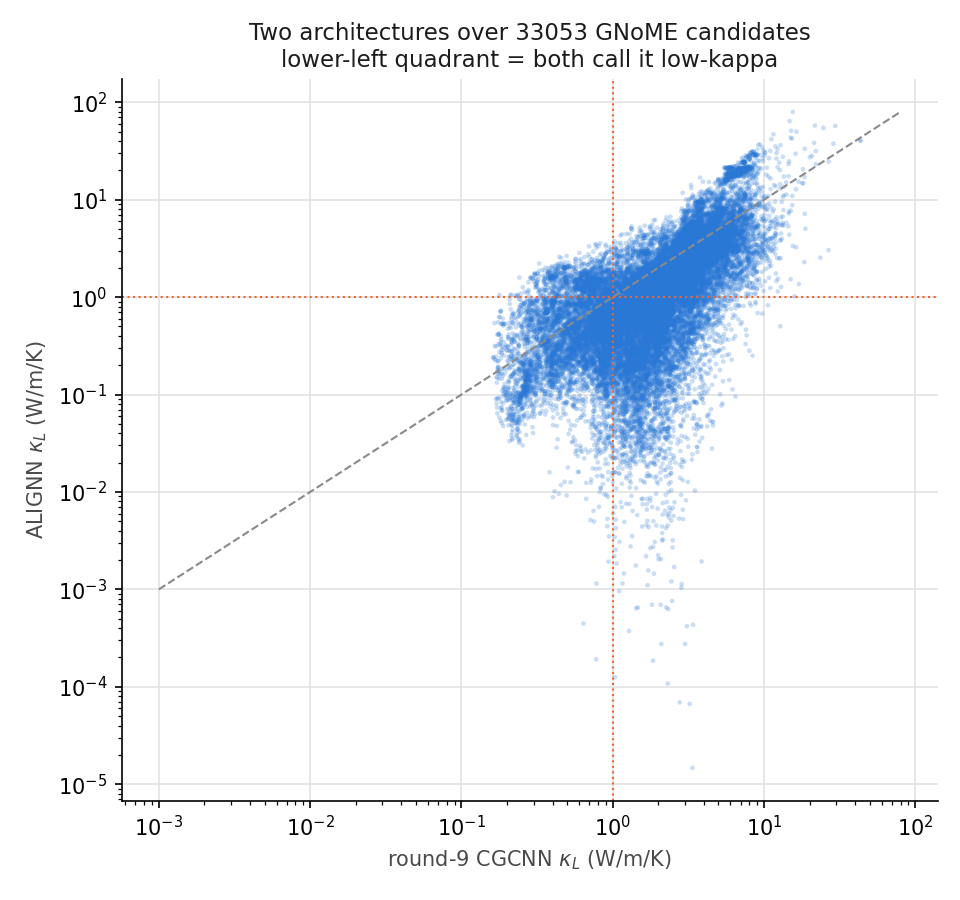
\includegraphics[width=0.70\linewidth]{../results/alignn/57_alignn_vs_r9_gnome.png}
\end{center}
\column{0.44\linewidth}
{\sffamily\footnotesize
All 33{,}118 candidates scored with ALIGNN --- 68 minutes, zero CIF failures.
Only the moduli change; the Slack chain and the structural constants are
identical, so nothing downstream can leak a difference.}

\vspace{5pt}
\Card{5.2cm}{CardBg}{CardRule}{%
  \sffamily\scriptsize
  \textbf{low-$\kappa$ call on 33{,}053 reliable candidates}\\[3pt]
  ALIGNN \dotfill 14{,}711 (44.5\%)\\
  round 9 \dotfill 7{,}262 (22.0\%)\\
  \textbf{both agree} \dotfill \textbf{6{,}006}\\
  Spearman $\rho$ \dotfill 0.723}

\vspace{4pt}
{\sffamily\scriptsize\color{Muted}
65 hit ALIGNN's $\sim$10$^{-3}$ GPa regression floor --- flagged, excluded.}
\end{columns}
\end{frame}

% -----------------------------------------------------------------------------
% OLD PAGE 39: What we found when we checked
% why removed: part divider
% -----------------------------------------------------------------------------
\PartSlide{SEVEN}{What we found when we checked}{Four evaluation failure modes, and three numbers that were wrong}

% -----------------------------------------------------------------------------
% OLD PAGE 40: The same candidates, four different answers
% why removed: four-model histogram (rebuilt as new 23)
% -----------------------------------------------------------------------------
\begin{frame}
\SlideHeader{22b \textperiodcentered\ THE SCREEN}{The same candidates, four different answers}

\begin{center}
\includegraphics[width=0.84\linewidth]{figures/kappa_dist_all_models.png}
\end{center}

\vspace{-3pt}
{\sffamily\scriptsize
Every model scores the identical 33{,}053 candidates through the identical
physics --- only $K$ and $G$ differ. Low-$\kappa$ counts: \textbf{16{,}130}
(CGCNN), \textbf{14{,}711} (ALIGNN), \textbf{17{,}034} (tree), \textbf{7{,}262}
(round 9). Three agree closely; round 9 sits far right and calls less than half
as many.}
\end{frame}

% -----------------------------------------------------------------------------
% OLD PAGE 42: Classifying the candidates: structural families
% why removed: families (not in outline)
% -----------------------------------------------------------------------------
\begin{frame}
\SlideHeader{22d \textperiodcentered\ THE SCREEN}{Classifying the candidates: structural families}

\begin{center}
\includegraphics[width=0.88\linewidth]{figures/families_all_models.png}
\end{center}

\vspace{-3pt}
{\sffamily\scriptsize
Non-oxides dominate, but \emph{how} much depends on the model: 68\% (CGCNN),
61\% (ALIGNN), 73\% (tree), 31\% (round 9). \textbf{The family ordering is
stable across all four; the absolute rate is not.}}
\end{frame}

% -----------------------------------------------------------------------------
% OLD PAGE 43: Every model this project has trained
% why removed: every model / AFLOW bars
% -----------------------------------------------------------------------------
\begin{frame}
\SlideHeader{22e \textperiodcentered\ THE SCREEN}{Every model this project has trained}

\begin{center}
\includegraphics[width=0.80\linewidth]{figures/model_comparison.png}
\end{center}

\vspace{-3pt}
{\sffamily\scriptsize
Bars absent where a model was never trained on that dataset --- not zero, not
measured. \textbf{The composition-only tree beats the CGCNN on AFLOW}
(0.0592 vs 0.1154) while losing on matbench: underfitting, not a limit of graph
networks, since the network's \emph{training} error there (0.103) exceeds the
tree's \emph{test} error.}
\end{frame}

% -----------------------------------------------------------------------------
% OLD PAGE 44: The screening metric was circular
% why removed: circular metric on AFLOW-AGL
% -----------------------------------------------------------------------------
\begin{frame}
\SlideHeader{23 \textperiodcentered\ FINDINGS}{The screening metric was circular}

\begin{columns}[T]
\column{0.52\linewidth}
\begin{center}
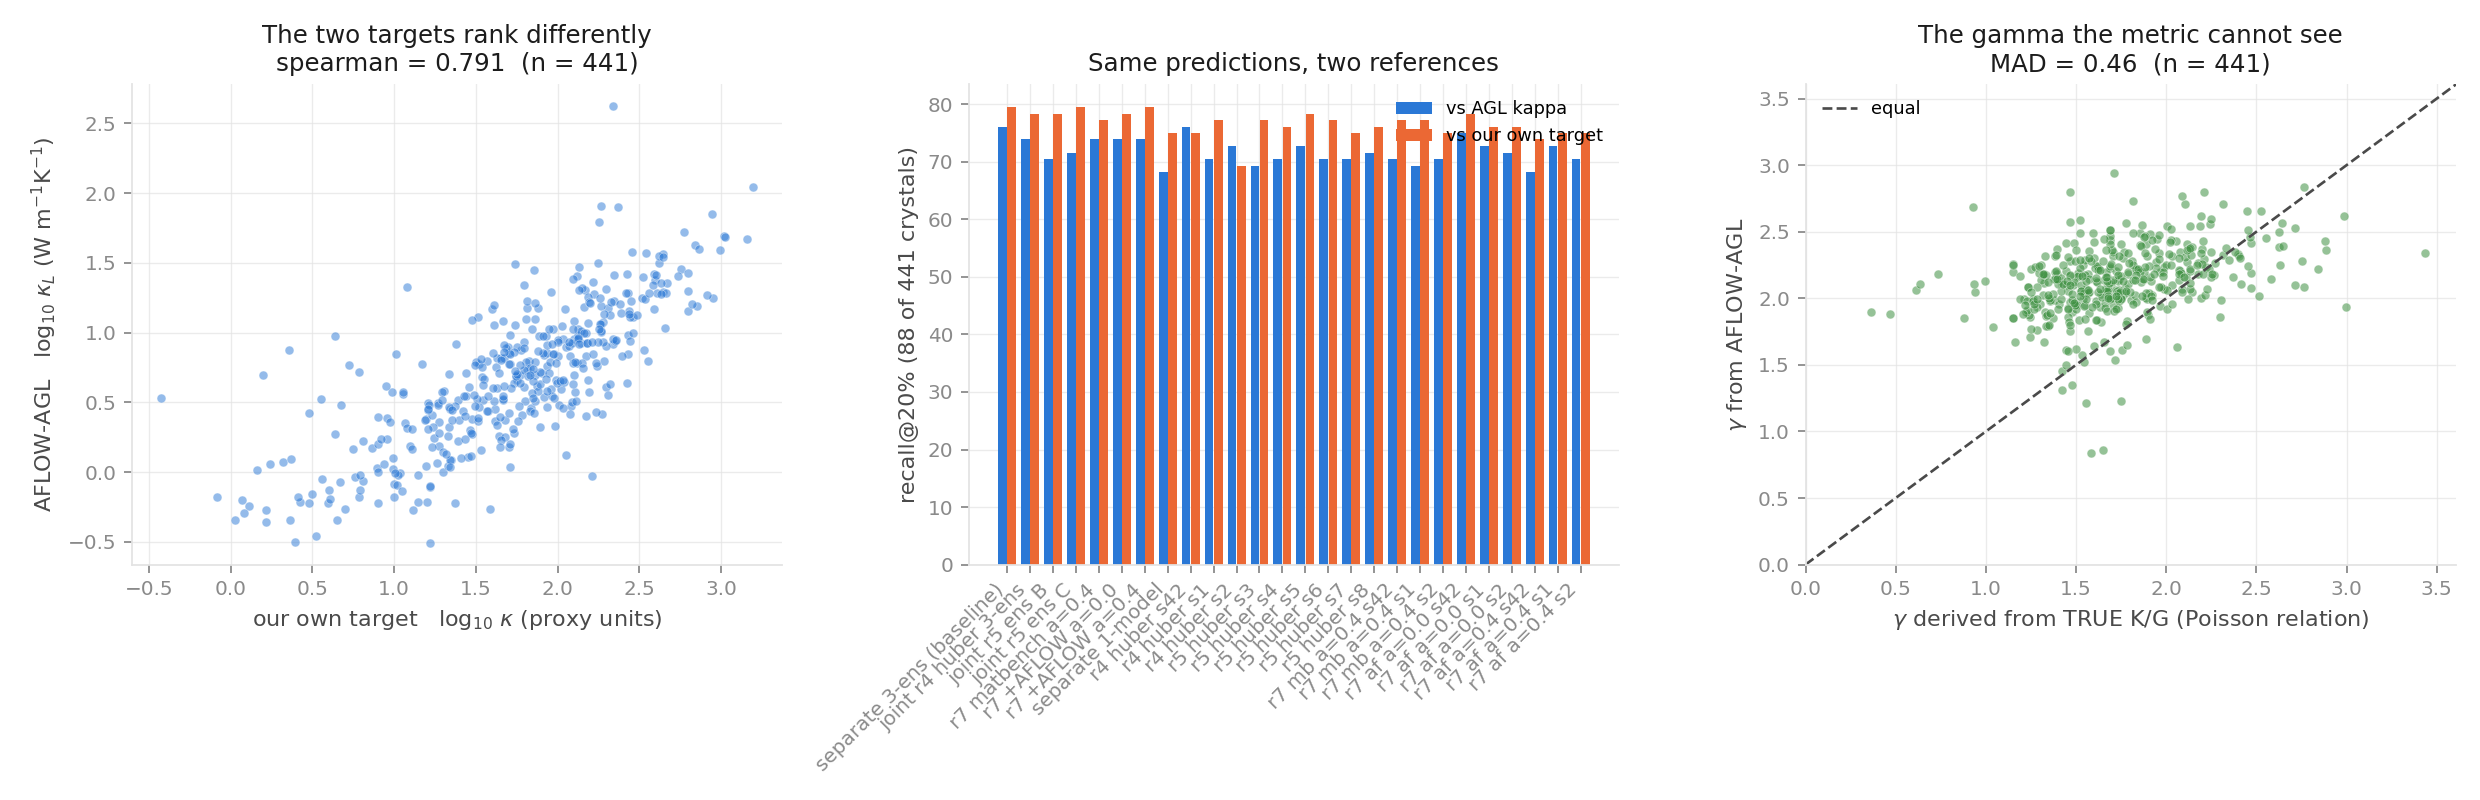
\includegraphics[width=\linewidth]{../results/cgcnn/agl_target/png/48_agl_vs_inhouse_target.png}
\end{center}
\column{0.44\linewidth}
{\sffamily\footnotesize
recall@10\% --- the fraction of the true lowest-$\kappa$ decile recovered ---
was scored against a reference that was \emph{this project's own} Slack chain on
matbench's true moduli, with $\gamma$ derived by the same relation the
prediction side uses.

\vspace{4pt}
Slack cancels. $\gamma$ cancels harder: \textbf{a model predicting a better
$\gamma$ scored worse}.}

\vspace{5pt}
\AccentCard{5.2cm}{SlideAmber}{%
  \sffamily\footnotesize
  Re-scored against AFLOW-AGL's independent $\kappa_L$ (441 matched crystals):
  recall@10\% fell \textbf{20.5 points}, Spearman $\rho$ fell \textbf{0.139}.}
\end{columns}

\Takeaway{The old metric actively penalised the one remaining lever. Quote
Spearman $\rho$ --- it is what transfers between targets ($\rho = 0.92$ across
26 runs); recall@10\% does not ($\rho = 0.20$).}
\end{frame}

% -----------------------------------------------------------------------------
% OLD PAGE 45: The misses are a fixed core, not variance
% why removed: fixed core of misses
% -----------------------------------------------------------------------------
\begin{frame}
\SlideHeader{24 \textperiodcentered\ FINDINGS}{The misses are a fixed core, not variance}

\begin{columns}[T]
\column{0.52\linewidth}
\begin{center}
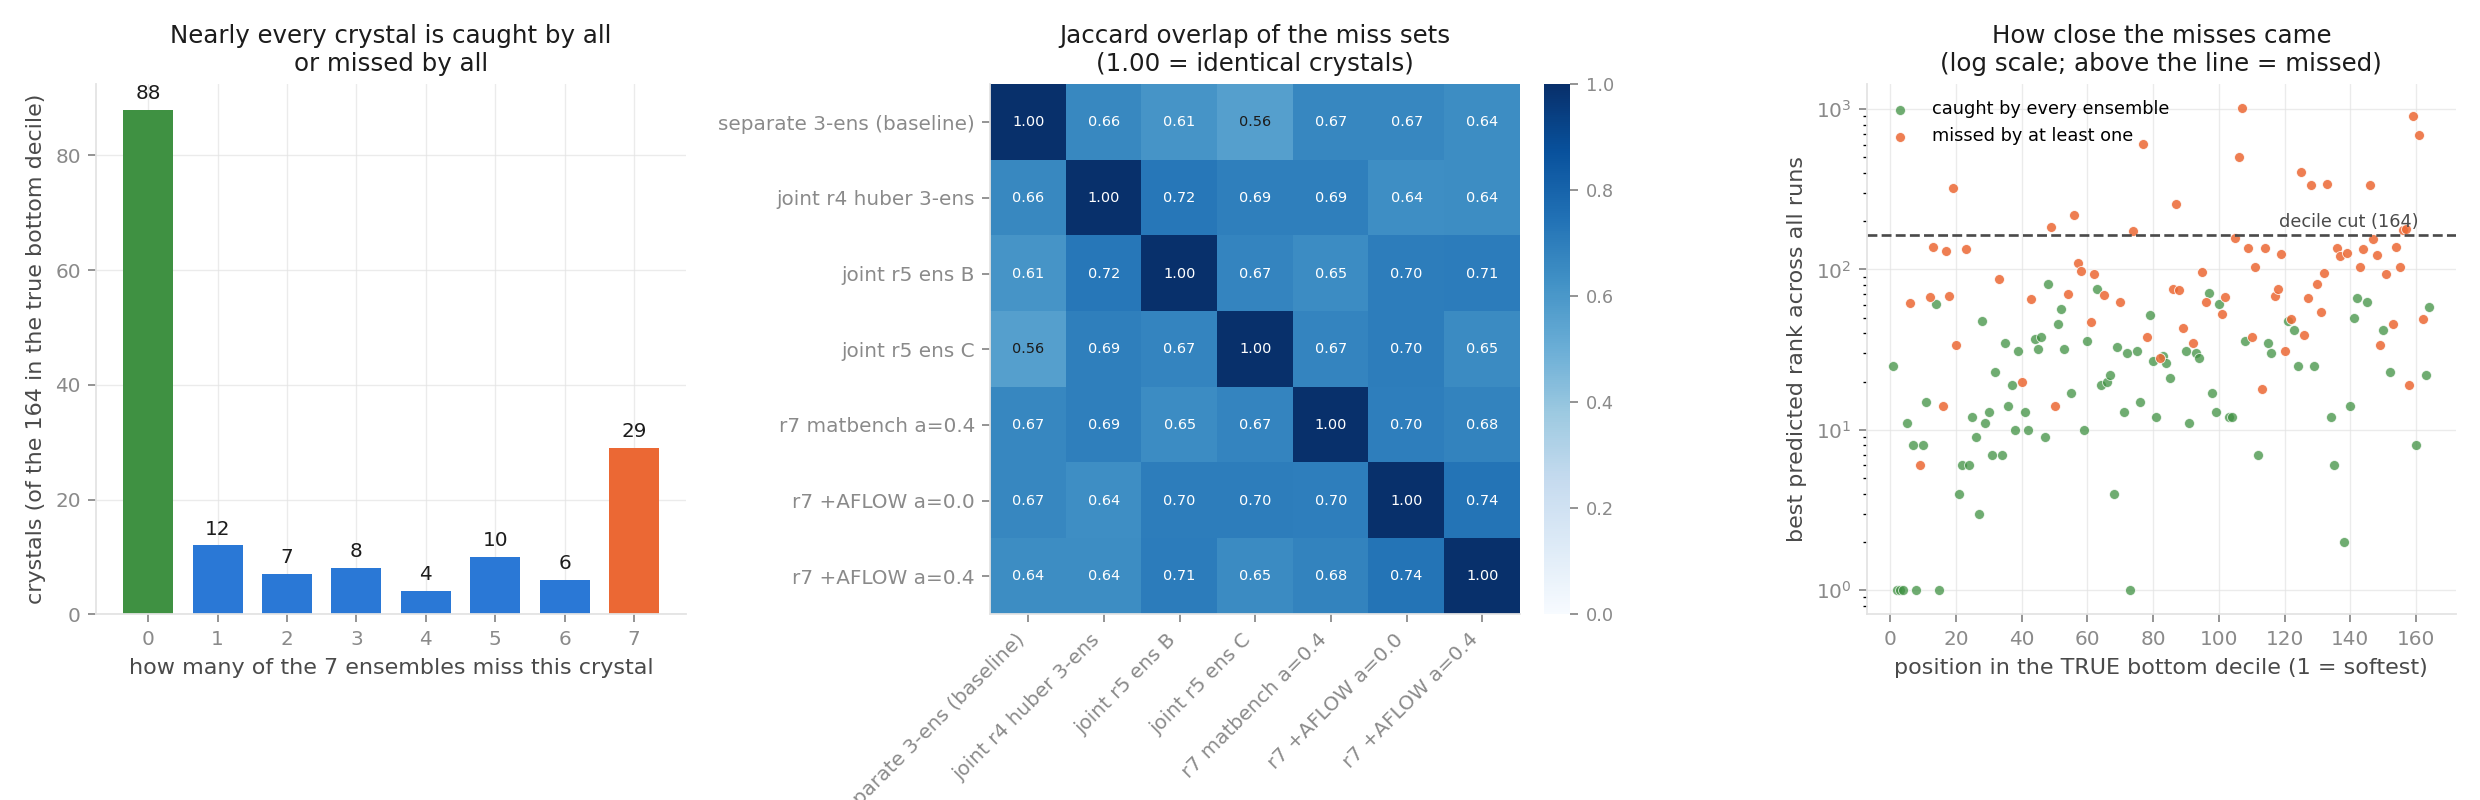
\includegraphics[width=\linewidth]{../results/cgcnn/decile_stability/png/47_missed_decile_stability.png}
\end{center}
\column{0.44\linewidth}
{\sffamily\footnotesize
Fingerprinting the saved prediction vectors collapsed 34 roster entries to
\textbf{26 distinct} runs --- eight were byte-identical duplicates.

\vspace{4pt}
Across those 26, recall spans \textbf{64.0--70.7\%}. \emph{Which} crystals are
missed is remarkably stable: \textbf{16 missed by all 26 runs}, 29 by all seven
ensembles, 65 never missed.}

\vspace{5pt}
\Card{5.2cm}{CardBg}{CardRule}{%
  \sffamily\scriptsize
  The 16 permanent misses: TmAg$_3$, MgAgAs, CeTe, Cs$_2$NaAlH$_6$, InSb, YSe
  and ten others --- median 4 sites, 9 of 16 cubic, never ranked better than
  173rd by anything.}
\end{columns}

\Takeaway{The ceiling is in the inputs, not the architecture. Seven rounds of
architecture work never moved it.}
\end{frame}

% -----------------------------------------------------------------------------
% OLD PAGE 46: A composition-only tree beats the network
% why removed: tree beats network on AFLOW
% -----------------------------------------------------------------------------
\begin{frame}
\SlideHeader{25 \textperiodcentered\ FINDINGS}{A composition-only tree beats the network}

\begin{columns}[T]
\column{0.50\linewidth}
\begin{center}
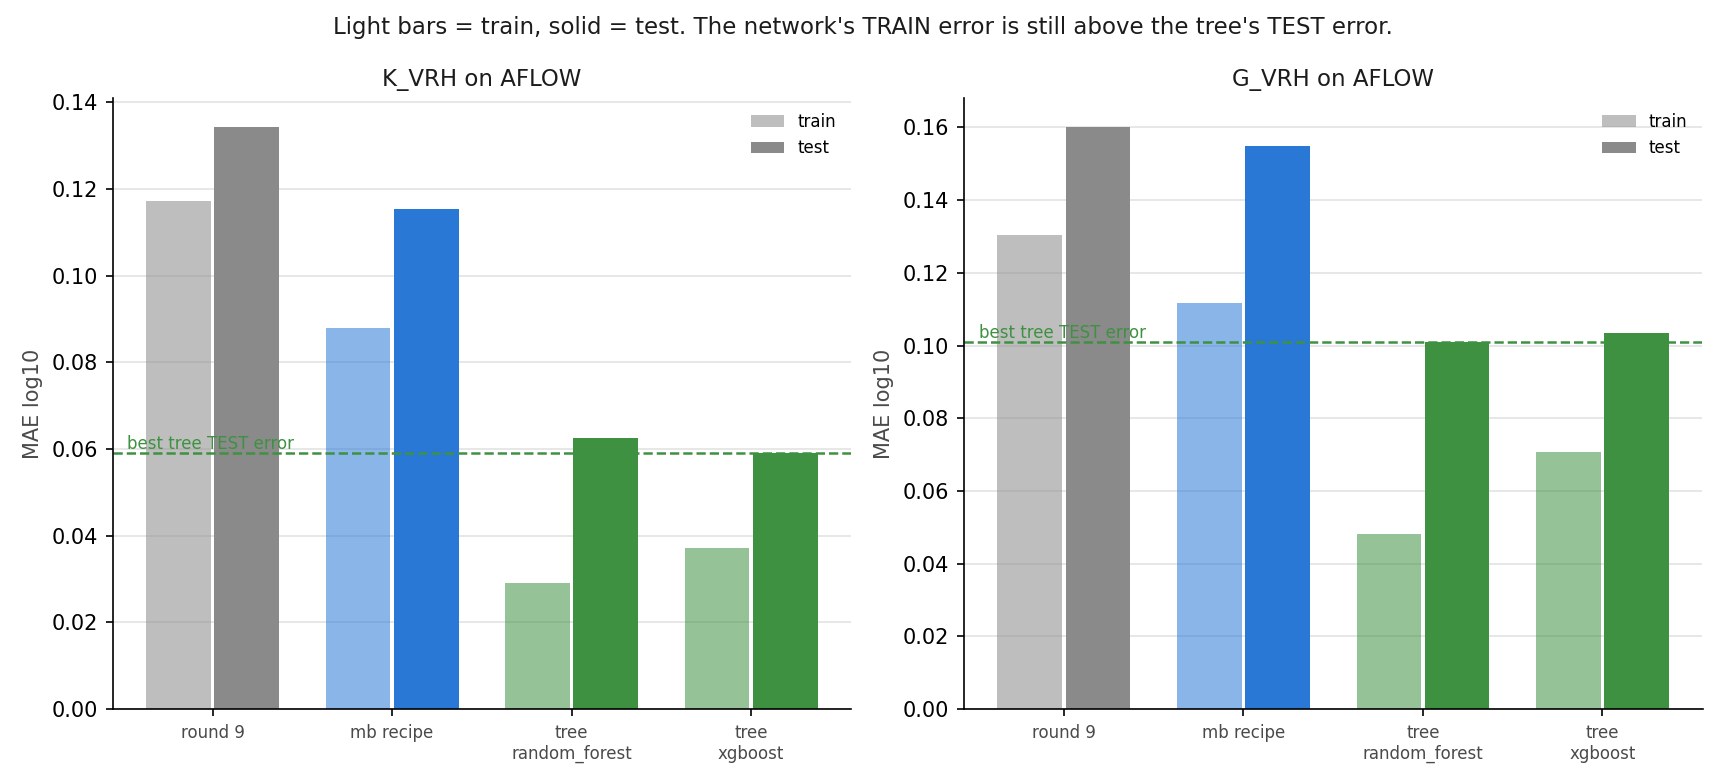
\includegraphics[width=\linewidth]{../results/cgcnn/underfitting/png/53_underfitting_verdict.png}
\end{center}
\column{0.46\linewidth}
{\sffamily\footnotesize
A decision tree on the composition-weighted mean of the same 92-dim element
table --- \textbf{no structure, no bonds} --- on the identical split:}

\vspace{4pt}
{\sffamily\scriptsize
\begin{tabular}{@{}lrr@{}}
\toprule
$K$ MAE $\log_{10}$ & tree & CGCNN \\
\midrule
matbench & 0.0868 & \textbf{0.0696} \\
AFLOW    & \textbf{0.0592} & 0.1154 \\
\bottomrule
\end{tabular}}

\vspace{5pt}
\AccentCard{5.2cm}{SlideAmber}{%
  \sffamily\footnotesize
  \textbf{The cause is underfitting, checked directly.}\\[3pt]
  Round 9's \emph{training} error on AFLOW $K$ is 0.103 --- worse than the
  tree's \emph{test} error of 0.059. A model that cannot fit its own training
  data is not out-generalised.}
\end{columns}

\Takeaway{Never report ``a decision tree beat our GNN'' without saying the GNN
was underfit. Composition memorisation was ruled out: only 9.6\% of AFLOW test
formulas appear in train, and excluding them moves the MAE by $<0.003$.}
\end{frame}

% -----------------------------------------------------------------------------
% OLD PAGE 47: The label noise everyone quotes was the wrong number
% why removed: matbench/AFLOW label noise
% -----------------------------------------------------------------------------
\begin{frame}
\SlideHeader{26 \textperiodcentered\ FINDINGS}{The label noise everyone quotes was the wrong number}

\begin{columns}[T]
\column{0.55\linewidth}
\begin{center}
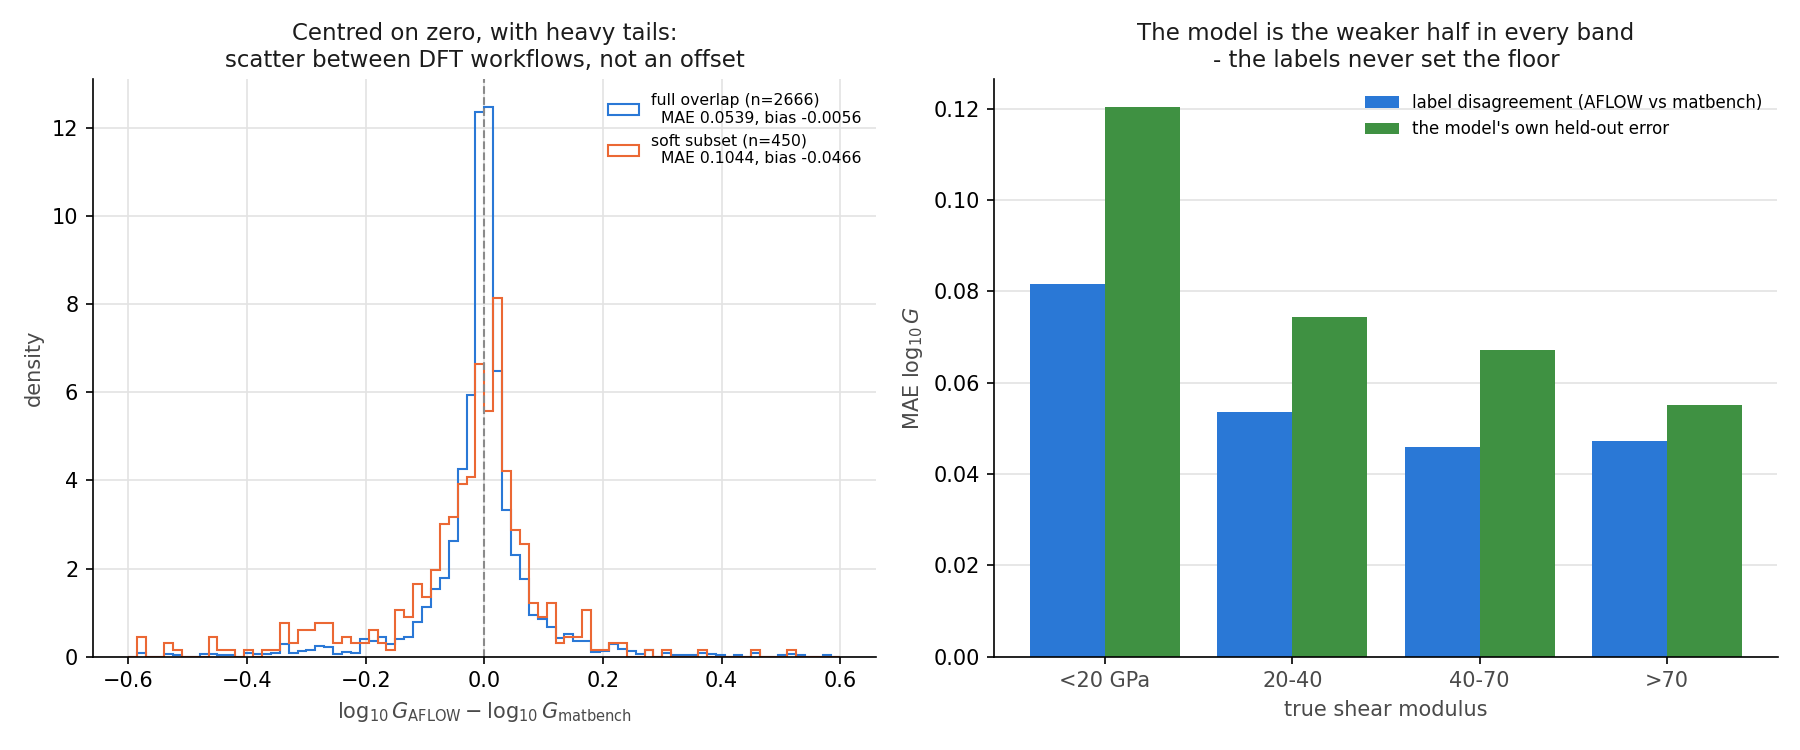
\includegraphics[width=\linewidth]{../results/cgcnn/59_cross_source_label_noise.png}
\end{center}
\column{0.41\linewidth}
{\sffamily\footnotesize
A single constant --- $|\Delta \log_{10} G| = 0.1085$ --- was hard-coded into
four scripts as \emph{the} matbench/AFLOW label noise, and divided by a
whole-test-set model error to argue the labels set the accuracy floor.}

\vspace{5pt}
\AccentCard{5.0cm}{SlideAmber}{%
  \sffamily\scriptsize
  \textbf{0.1085 is the \emph{soft subset's} number.}\\[3pt]
  Full overlap (n = 2{,}666): \textbf{0.0539}\\[2pt]
  Population-matched ratio: 0.69, not 1.39\\[2pt]
  Per stiffness band the \emph{model's} error exceeds the label disagreement in
  \textbf{all four}.}


\end{columns}

\Takeaway{The network, not the labels, is the weaker half.}
\end{frame}

% -----------------------------------------------------------------------------
% OLD PAGE 48: Where a cross-model disagreement actually lives
% why removed: cross-model disagreement
% -----------------------------------------------------------------------------
\begin{frame}
\SlideHeader{27 \textperiodcentered\ FINDINGS}{Where a cross-model disagreement actually lives}

\begin{columns}[T]
\column{0.56\linewidth}
\begin{center}
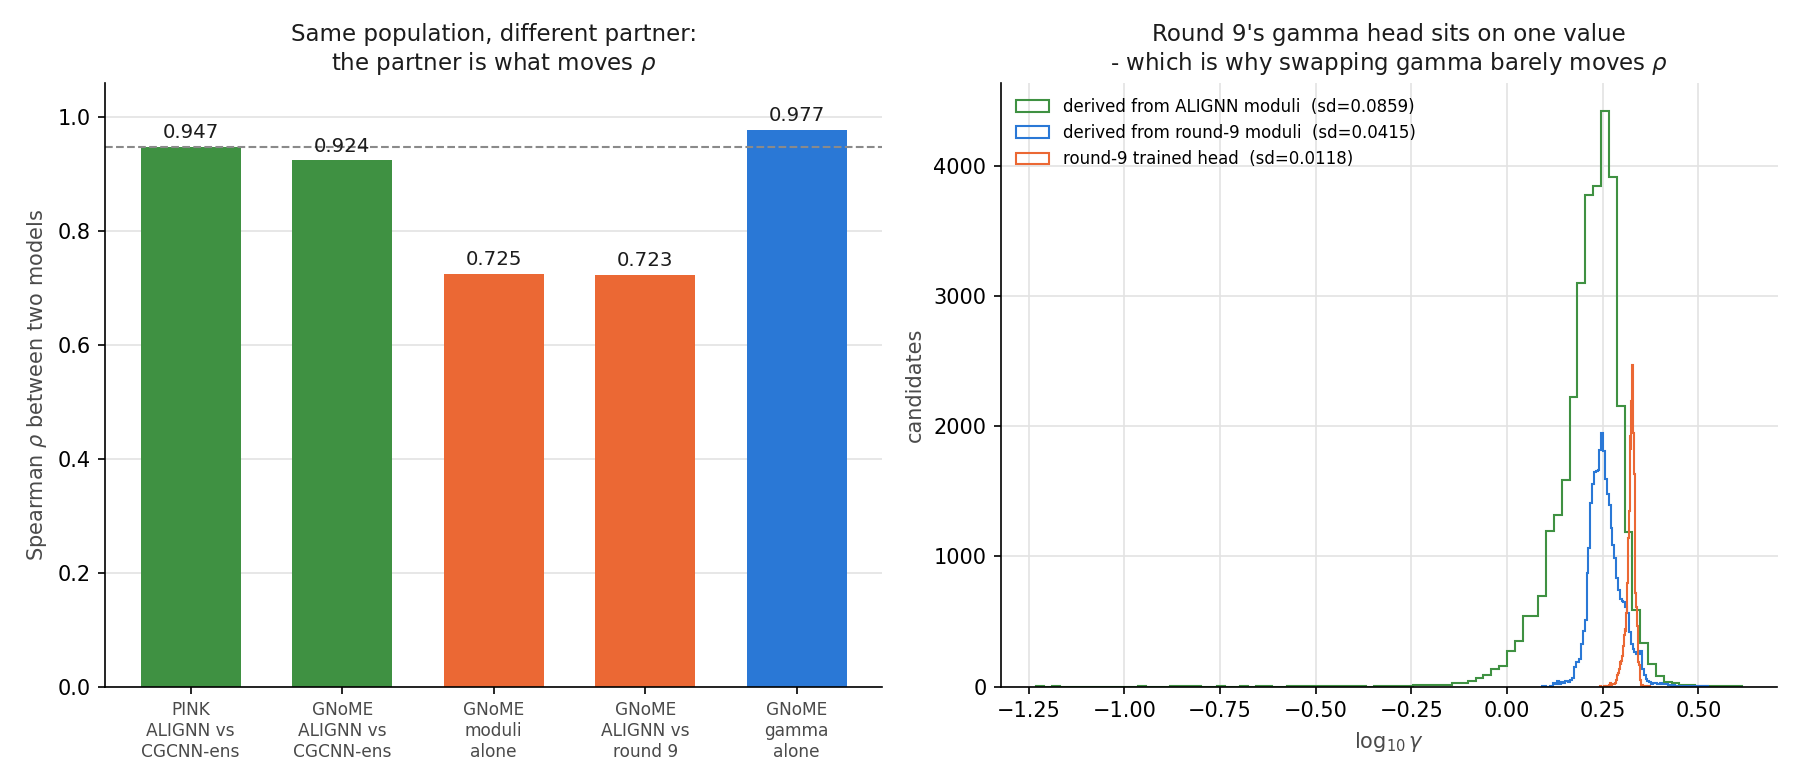
\includegraphics[width=\linewidth]{../results/alignn/58_rho_decomposition.png}
\end{center}
\column{0.40\linewidth}
{\sffamily\footnotesize
Agreement between ALIGNN and the CGCNN ensemble is $\rho = 0.947$ on the PINK
set but only 0.723 against round 9 on GNoME. Two explanations were plausible:
the exotic GNoME chemistry, or the partner model.}

\vspace{5pt}
{\sffamily\scriptsize
\begin{tabular}{@{}lr@{}}
\toprule
population cost (PINK $\rightarrow$ GNoME) & $-0.023$ \\
partner cost (ens.\ $\rightarrow$ round 9) & $\mathbf{-0.201}$ \\
\midrule
moduli alone & 0.725 \\
$\gamma$ alone & 0.977 \\
\bottomrule
\end{tabular}}

\vspace{4pt}
{\sffamily\scriptsize\color{Muted}
Holding the partner fixed, GNoME's chemistry costs almost nothing. Swapping the
partner costs nine times more --- and it is entirely the moduli.}
\end{columns}

\Takeaway{Round 9's $\gamma$ head collapsed to near-constant (sd
$0.0118$, rank correlation $-0.028$). A constant barely perturbs a
\emph{ranking} --- invisible to $\rho$, still wrong in absolute $\kappa$.}
\end{frame}

% -----------------------------------------------------------------------------
% OLD PAGE 49: The joint model worked better than the record said
% why removed: joint model
% -----------------------------------------------------------------------------
\begin{frame}
\SlideHeader{28 \textperiodcentered\ FINDINGS}{The joint model worked better than the record said}

\begin{columns}[T]
\column{0.55\linewidth}
\begin{center}
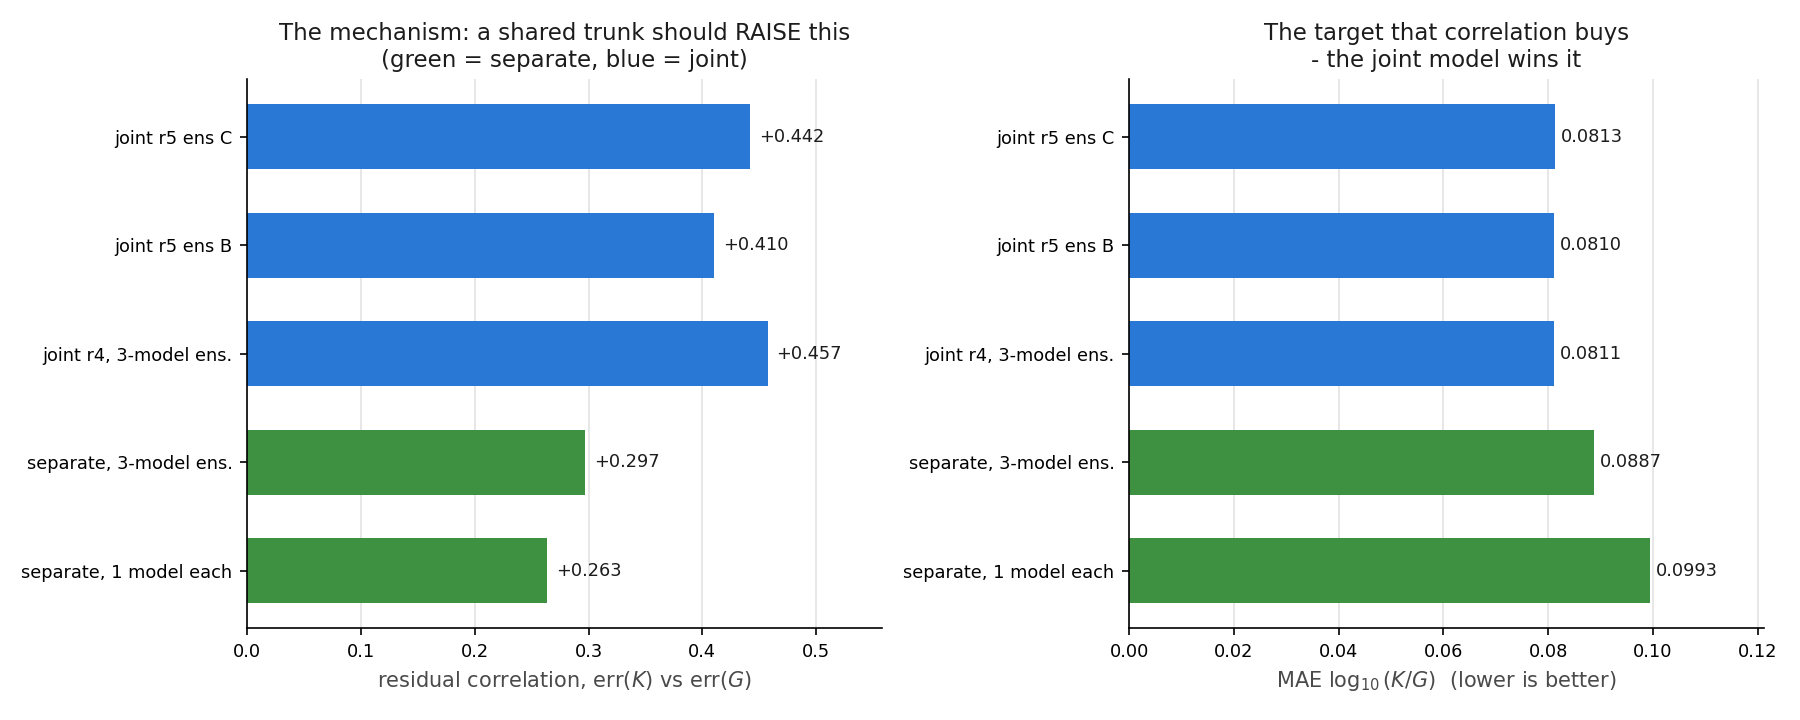
\includegraphics[width=\linewidth]{../results/cgcnn/60_residual_corr_table.png}
\end{center}
\column{0.41\linewidth}
{\sffamily\footnotesize
$\kappa_L$ depends on $K$ and $G$ only through their \emph{ratio}, and in log
space a ratio is a difference --- so independent errors \textbf{add}. A shared
trunk should make them correlate instead.}

\vspace{4pt}
{\sffamily\scriptsize
\begin{tabular}{@{}lrr@{}}
\toprule
& corr & MAE $\log_{10}(K/G)$ \\
\midrule
separate, 1 each & $+0.263$ & 0.0993 \\
separate, 3-ens  & $+0.297$ & 0.0887 \\
\textbf{joint 3-ens} & $\mathbf{+0.457}$ & \textbf{0.0811} \\
\bottomrule
\end{tabular}}

\vspace{4pt}
{\sffamily\scriptsize\color{Muted}
A published table had labelled the first two columns ``separate'' and
``joint'' --- so it contained no joint model at all. The real correlation is
1.5$\times$ the ensemble's.}
\end{columns}

\Takeaway{The mechanism worked; it is paid for in per-modulus accuracy.}
\end{frame}

% -----------------------------------------------------------------------------
% OLD PAGE 50: The audit
% why removed: part divider
% -----------------------------------------------------------------------------
\PartSlide{EIGHT}{The audit}{Every number in this deck, recomputed from its source}

% -----------------------------------------------------------------------------
% OLD PAGE 55: Three traps the rebuild walked into
% why removed: three traps
% -----------------------------------------------------------------------------
\begin{frame}
\SlideHeader{33 \textperiodcentered\ AUDIT}{Three traps the rebuild walked into}

\begin{columns}[T]
\column{0.31\linewidth}
\AccentCard{3.75cm}{SlideAmber}{%
  \sffamily\scriptsize
  \textbf{1. A tie at the 10\% cut}\\[3pt]
  \texttt{mb-09580} and \texttt{mb-00161} have identical labels ($K$ 17, $G$ 9
  GPa) and share 164th place. The original step kept one and counted
  \textbf{108} hits; the rebuild kept the other and counted \textbf{109}.\\[3pt]
  Both are right. The check now accepts the whole range over every tie
  choice.\par}
\column{0.31\linewidth}
\AccentCard{3.75cm}{SlideRed}{%
  \sffamily\scriptsize
  \textbf{2. numpy changed how it sorts ties}\\[3pt]
  Matbench moduli are whole GPa, so many crystals tie. numpy 2's fast (AVX2)
  sort orders ties differently from numpy 1.26: \textbf{41 MISMATCH + 23
  close}, with no bug anywhere.\\[3pt]
  Forcing the old sort path (\texttt{NPY\_DISABLE\_CPU\_FEATURES=AVX2}):
  \textbf{0}.\par}
\column{0.31\linewidth}
\AccentCard{3.75cm}{SlideBlue}{%
  \sffamily\scriptsize
  \textbf{3. A label, not a number}\\[3pt]
  Two $\gamma$ models (gamma3, round 8) were listed as tested on the 835-crystal
  split. They were tested on the AFLOW $\gamma$ set: \textbf{1{,}460} crystals,
  1{,}022 for training.\\[3pt]
  The numbers were right; the description of them was not.\par}
\end{columns}

\Takeaway{None of the three changes a conclusion --- but two would have shown up
as MISMATCH and sent someone hunting a bug that does not exist. An audit has to
\emph{explain} its differences, not only count them.}
\end{frame}

% -----------------------------------------------------------------------------
% OLD PAGE 56: The DFT list
% why removed: part divider
% -----------------------------------------------------------------------------
\PartSlide{NINE}{The DFT list}{15 crystals handed over for a phonon-DFT $\kappa_L$}

% -----------------------------------------------------------------------------
% OLD PAGE 61: What we cannot reproduce
% why removed: what we cannot reproduce (one line -> summary)
% -----------------------------------------------------------------------------
\begin{frame}[plain]
\vspace{0.9cm}
\begin{center}
{\color{SlideAmber}\bfseries\sffamily\large PAPER FIGURES 9 AND 10}\\[8pt]
{\color{white}\bfseries\headingfont\fontsize{25}{30}\selectfont
  What we cannot reproduce}\\[12pt]
\begin{minipage}{0.80\linewidth}
{\color{Subtle}\sffamily\footnotesize
The paper's last two figures are \textbf{DFT phonon calculations} on
Ag$_3$Te$_4$X --- primitive structures, phonon dispersions, then $\kappa_L$
against temperature, cumulative $\kappa_L$, specific heat, mode group
velocities, scattering phase space and scattering rates.\\[8pt]
Producing them needs a full DFT plus finite-displacement phonon workflow with
\textbf{third-order force constants}, on materials this project has never
computed --- days of DFT per material, and a different toolchain from anything
here.\\[8pt]
{\color{white}No stand-in is drawn for them.} They are the same missing
ground-truth gap the 15-crystal $\kappa_L$ DFT list (Part 9) starts to close.}
\end{minipage}
\end{center}
\end{frame}

% =============================================================================
%  PART B - originals of frames that were merged or rewritten
% =============================================================================

% -----------------------------------------------------------------------------
% OLD PAGE 1: ALIGNN and the PINK Pipeline
% now feeds new slide(s): 1
% -----------------------------------------------------------------------------
\begin{frame}[plain]
\vspace{0.9cm}
\begin{center}
{\color{LightBlue}\bfseries\sffamily\large FINDINGS AND METHOD}\\[6pt]
{\color{white}\bfseries\headingfont\fontsize{32}{38}\selectfont
  ALIGNN and the PINK Pipeline}\\[6pt]
{\color{Subtle}\sffamily\large
  A second architecture, the full 554{,}054-material screen,\\
  and what changed when every claim was checked}\\[16pt]
\begin{tikzpicture}[node distance=3.5mm,
  pill/.style={rounded corners=4pt, fill=Navy!60, draw=LightBlue!40,
               line width=0.5pt, minimum height=0.8cm, align=center,
               inner sep=5pt, font=\sffamily\bfseries\scriptsize\color{white}},
  arr/.style={font=\color{LightBlue}\normalsize}]
  \node[pill] (n1) {CIF};
  \node[arr, right=of n1] (a1) {$\rightarrow$};
  \node[pill, right=of a1] (n2) {atom graph\\+ line graph};
  \node[arr, right=of n2] (a2) {$\rightarrow$};
  \node[pill, right=of a2] (n3) {$K$, $G$};
  \node[arr, right=of n3] (a3) {$\rightarrow$};
  \node[pill, right=of a3] (n4) {Slack model};
  \node[arr, right=of n4] (a4) {$\rightarrow$};
  \node[pill, right=of a4] (n5) {$\kappa_L$};
\end{tikzpicture}
\end{center}
\end{frame}

% -----------------------------------------------------------------------------
% OLD PAGE 3: What PINK does, in one slide
% now feeds new slide(s): 2
% -----------------------------------------------------------------------------
\begin{frame}
\SlideHeader{01 \textperiodcentered\ THE PIPELINE}{What PINK does, in one slide}

\begin{columns}[T]
\column{0.54\linewidth}
{\sffamily\footnotesize
PINK (Liu \textit{et al.}, \textit{J. Mater. Inf.} 2025) predicts \textbf{lattice
thermal conductivity} $\kappa_L$ straight from a CIF file, without solving the
phonon Boltzmann transport equation.

\vspace{4pt}
It does that in two stages. A crystal graph network predicts the two elastic
moduli; a closed-form physical model turns those into $\kappa_L$. The physics
stage has no free parameters --- it is the Slack model, not a fit.}

\vspace{5pt}
\Card{6.3cm}{CardBg}{CardRule}{%
  \sffamily\footnotesize
  \textbf{Why this is worth doing}\\[3pt]
  A full DFT + PBTE calculation of $\kappa_L$ takes days per material. This
  takes about a sixth of a second. That is the difference between checking a
  handful of candidates and screening half a million.}

\column{0.42\linewidth}
{\sffamily\footnotesize\color{Muted} The two stages:}\\[4pt]
\begin{tikzpicture}[node distance=4mm,
  box/.style={rounded corners=4pt, fill=CardBg, draw=CardRule, line width=0.7pt,
              text width=4.5cm, align=left, inner sep=6pt,
              font=\sffamily\scriptsize\color{SlideInk}},
  arr/.style={font=\color{SlideBlue}\small}]
  \node[box] (b1) {\textbf{Stage 1 --- learned}\\ CIF $\rightarrow$ graph network
                   $\rightarrow$ bulk modulus $K$, shear modulus $G$};
  \node[arr, below=of b1] (a1) {$\downarrow$};
  \node[box, below=of a1] (b2) {\textbf{Stage 2 --- physics}\\ $K$, $G$
                   $\rightarrow$ Poisson ratio $\rightarrow$ sound velocity,
                   Debye temperature, Gr\"uneisen $\gamma$ $\rightarrow$ $\kappa_L$};
\end{tikzpicture}
\end{columns}

\Takeaway{The network never sees a thermal conductivity. It learns elasticity;
the physics does the rest.}
\end{frame}

% -----------------------------------------------------------------------------
% OLD PAGE 4: The paper's own Figure 1
% now feeds new slide(s): 3
% -----------------------------------------------------------------------------
\begin{frame}
\SlideHeader{01b \textperiodcentered\ THE PIPELINE}{The paper's own Figure 1}

\begin{center}
\includegraphics[width=0.83\linewidth]{figures/paper_fig1_workflow.png}
\end{center}

\vspace{-2pt}
{\sffamily\scriptsize
Reproduced from Liu \textit{et al.}, \textit{J.\ Mater.\ Inf.} 2025, 5, 12
(CC BY 4.0). \textbf{Blue} the input CIF; \textbf{yellow} the only learned step;
\textbf{purple and green} the closed-form physics; \textbf{red} the answer. The
boxed equation is the one this project reports --- note $\kappa_L \propto
e^{-\gamma}$, an \emph{exponential} dependence on the Gr\"uneisen parameter.}
\end{frame}

% -----------------------------------------------------------------------------
% OLD PAGE 5: What this project added
% now feeds new slide(s): 4
% -----------------------------------------------------------------------------
\begin{frame}
\SlideHeader{02 \textperiodcentered\ THE PIPELINE}{What this project added}

\begin{columns}[T]
\column{0.48\linewidth}
\AccentCard{6.4cm}{SlideBlue}{%
  \sffamily\footnotesize
  \textbf{A second architecture}\\[2pt]
  ALIGNN, on the identical split, so the two compare without caveats. It
  beats the CGCNN ensemble on both moduli.\par}
\vspace{4pt}
\AccentCard{6.4cm}{SlideGreen}{%
  \sffamily\footnotesize
  \textbf{The full screen, twice}\\[2pt]
  All 33{,}118 GNoME candidates scored by both architectures --- the paper's
  headline experiment, rerun.\par}
\vspace{4pt}
\AccentCard{6.4cm}{SlideAmber}{%
  \sffamily\footnotesize
  \textbf{Validation against measurement}\\[2pt]
  45 materials with experimentally measured $\kappa_L$, not model-vs-model.\par}

\column{0.48\linewidth}
\AccentCard{5.6cm}{Muted}{%
  \sffamily\footnotesize
  \textbf{And --- the part that took longest ---}\\[2pt]
  every headline claim re-checked against the artefacts that produced it.
  Four evaluation failure modes were found, each of which inflates reported
  performance. Three numbers already written down turned out to be wrong.\par}

\vspace{6pt}
{\sffamily\footnotesize
Parts 6--7 are those checks. Part 8 recomputes every stored metric from scratch
(0 mismatches); Part 9 is the 15-crystal list now going to DFT.\par}
\end{columns}

\Takeaway{Two architectures agreeing is evidence. Two architectures agreeing
because they share a mistake is not --- so most of the work went into telling
those apart.}
\end{frame}

% -----------------------------------------------------------------------------
% OLD PAGE 7: Why a second architecture at all
% now feeds new slide(s): 6
% -----------------------------------------------------------------------------
\begin{frame}
\SlideHeader{03 \textperiodcentered\ CIF TO GRAPH}{Why a second architecture at all}

{\sffamily\footnotesize
A single model that scores well can be right for the wrong reason. Two models
that share only the training data and the physics --- not the architecture ---
give an independent check: where they agree, the signal is unlikely to be an
artefact of either one.

\vspace{4pt}
ALIGNN was chosen because its difference from CGCNN is \textbf{physically
motivated rather than incidental}. It is not a bigger CGCNN or a differently
tuned one. It sees something CGCNN structurally cannot: \textbf{bond angles}.}

\vspace{6pt}
\begin{columns}[T]
\column{0.47\linewidth}
\Card{5.6cm}{CardBg}{CardRule}{%
  \sffamily\footnotesize
  \textbf{What CGCNN encodes}\\[3pt]
  Which atoms exist, which are bonded, and \emph{how far apart} they are.
  A pure two-body description.}
\column{0.47\linewidth}
\Card{5.6cm}{CardBg}{CardRule}{%
  \sffamily\footnotesize
  \textbf{What ALIGNN adds}\\[3pt]
  The \emph{angles} between bonds --- a three-body term. Elastic response to
  shear depends on how bonds resist \emph{bending}, not only stretching.}
\end{columns}

\Takeaway{Shear modulus is a bond-bending property. A model blind to angles is
being asked to infer it indirectly.}
\end{frame}

% -----------------------------------------------------------------------------
% OLD PAGE 8: Step 1 - the CIF, and finding neighbours
% now feeds new slide(s): 7
% -----------------------------------------------------------------------------
\begin{frame}
\SlideHeader{04 \textperiodcentered\ CIF TO GRAPH}{Step 1 --- the CIF, and finding neighbours}

\begin{columns}[T]
\column{0.50\linewidth}
{\sffamily\footnotesize
Identical to CGCNN's start: a CIF gives lattice vectors, fractional coordinates
and the element at each site. Neighbours come from a \textbf{periodic distance
search}, so an atom near a face still finds those across the boundary.}

\vspace{5pt}
\Card{6.0cm}{CardBg}{CardRule}{%
  \sffamily\footnotesize
  \textbf{The two settings that define the graph}\\[3pt]
  \texttt{cutoff = 5.0} \AA\ --- the radius within which a neighbour counts\\[2pt]
  \texttt{max\_neighbors = 12} --- the cap per atom\\[3pt]
  {\color{Muted}Read from the trained model's own config --- building 8.0 \AA\
  graphs for a 5.0 \AA\ model would feed it an unseen neighbourhood.}}

\column{0.46\linewidth}
{\sffamily\footnotesize\color{Muted} What comes out of this step:}\\[3pt]
\begin{tabular}{@{}ll@{}}
\toprule
\footnotesize quantity & \footnotesize becomes \\
\midrule
\footnotesize element at site $i$ & \footnotesize node feature $\mathbf{v}_i$ \\
\footnotesize bond $i \rightarrow j$ & \footnotesize edge $e_{ij}$ \\
\footnotesize distance $r_{ij}$ & \footnotesize edge feature \\
\footnotesize angle $\theta_{jik}$ & \footnotesize \textbf{ALIGNN only} \\
\bottomrule
\end{tabular}

\vspace{6pt}
{\sffamily\footnotesize
Node features come from the same 92-dimensional element table CGCNN uses
(\texttt{atom\_features = cgcnn} in the config), so the two architectures start
from identical chemistry.}
\end{columns}
\end{frame}

% -----------------------------------------------------------------------------
% OLD PAGE 9: Step 2 - one crystal becomes two graphs
% now feeds new slide(s): 7
% -----------------------------------------------------------------------------
\begin{frame}
\SlideHeader{05 \textperiodcentered\ CIF TO GRAPH}{Step 2 --- one crystal becomes \emph{two} graphs}

\begin{center}
\includegraphics[width=0.97\linewidth]{figures/alignn_line_graph.png}
\end{center}

\vspace{-2pt}
{\sffamily\footnotesize
\textbf{A} the real motif: a centre atom, its neighbours, and the angles between
the bonds. \quad
\textbf{B} the \textbf{atom graph} $\mathcal{G}$ --- atoms are nodes, bonds are
edges. This is exactly what CGCNN builds, and where CGCNN stops. \quad
\textbf{C} the \textbf{line graph} $\mathcal{L}$ --- every \emph{bond} of
$\mathcal{G}$ becomes a \emph{node}, and two bonds sharing an atom are joined by
an edge that carries the angle between them.}

\Takeaway{The line graph is a graph \emph{of the bonds}; its edges are angles.}
\end{frame}

% -----------------------------------------------------------------------------
% OLD PAGE 10: The same thing on a real file: NaCl
% now feeds new slide(s): 8
% -----------------------------------------------------------------------------
\begin{frame}
\SlideHeader{05b \textperiodcentered\ CIF TO GRAPH}{The same thing on a real file: NaCl}

\begin{center}
\includegraphics[width=0.97\linewidth]{figures/nacl_alignn_graphs.png}
\end{center}

\vspace{-2pt}
\vspace{-2pt}
\begin{columns}[T]
\column{0.44\linewidth}
{\sffamily\scriptsize
Computed from \texttt{nacl.cif} at \textbf{ALIGNN's own} settings --- cutoff
5.0 \AA, max 12 neighbours, from the trained model's config.

\vspace{3pt}
A \textbf{bond is two things at once}: an \emph{edge} of $\mathcal{G}$, a
\emph{node} of $\mathcal{L}$.}

\column{0.53\linewidth}
{\sffamily\scriptsize
\begin{tabular}{@{}llll@{}}
\toprule
 & node & edge & edge feature \\
\midrule
$\mathcal{G}$ & atom (8) & bond (96) & length $r_{ij}$ \\
$\mathcal{L}$ & bond (96) & angle (528) & angle $\theta_{jik}$ \\
\bottomrule
\end{tabular}}

\vspace{3pt}
{\sffamily\scriptsize
12 nbrs $\rightarrow \binom{12}{2} = 66$ angles, $8 \times 66 = 528$, so
$528/96 = \mathbf{5.5\times}$ the edges. Panel \textbf{C} shows site 0 only.}
\end{columns}
\end{frame}

% -----------------------------------------------------------------------------
% OLD PAGE 11: Why the line graph is the right construction
% now feeds new slide(s): 7
% -----------------------------------------------------------------------------
\begin{frame}
\SlideHeader{06 \textperiodcentered\ CIF TO GRAPH}{Why the line graph is the right construction}

\begin{columns}[T]
\column{0.50\linewidth}
{\sffamily\footnotesize
A message-passing network updates a node from its neighbours. On the atom graph
alone, the only geometric quantity available to a message is the bond
\emph{length} $r_{ij}$ --- there is nowhere for an angle to live, because an
angle is a property of a \emph{pair} of bonds, not of one.

\vspace{4pt}
Promoting bonds to nodes solves that exactly. In $\mathcal{L}$, a pair of bonds
is an \emph{edge}, and an edge is precisely where a feature can be attached.}

\vspace{5pt}
\Card{6.0cm}{CardBg}{CardRule}{%
  \sffamily\footnotesize
  \textbf{Counting the geometry}\\[3pt]
  An atom with $n$ neighbours contributes $n$ nodes to $\mathcal{L}$ and
  $\binom{n}{2}$ angle edges. At \texttt{max\_neighbors = 12} that is up to
  66 angles per atom --- the reason ALIGNN costs more per structure than
  CGCNN does.}

\column{0.46\linewidth}
{\sffamily\footnotesize\color{Muted} Angle encoding:}\\[3pt]
{\sffamily\footnotesize
The angle is fed as $\cos\theta_{jik}$ expanded on a radial basis, the same way
distances are. Using the cosine rather than the angle keeps the feature smooth
where it matters and avoids a discontinuity at $0$ and $\pi$.}

\vspace{6pt}
\Card{5.4cm}{CardBg}{CardRule}{%
  \sffamily\footnotesize
  \textbf{A sanity check}\\[3pt]
  A cubic cell and a sheared one with identical bond lengths are
  \emph{indistinguishable} to a two-body descriptor, and distinct to ALIGNN.}
\end{columns}
\end{frame}

% -----------------------------------------------------------------------------
% OLD PAGE 12: Step 3 - the ALIGNN layer alternates between them
% now feeds new slide(s): 9
% -----------------------------------------------------------------------------
\begin{frame}
\SlideHeader{07 \textperiodcentered\ CIF TO GRAPH}{Step 3 --- the ALIGNN layer alternates between them}

\begin{columns}[T]
\column{0.52\linewidth}
{\sffamily\footnotesize
One ALIGNN layer is two coupled updates, run in order:}

\vspace{5pt}
\begin{tikzpicture}[node distance=4.5mm,
  box/.style={rounded corners=4pt, fill=CardBg, draw=CardRule, line width=0.7pt,
              text width=5.6cm, align=left, inner sep=6pt,
              font=\sffamily\scriptsize\color{SlideInk}},
  arr/.style={font=\color{SlideBlue}\small}]
  \node[box] (b1) {\textbf{1. Update on the line graph $\mathcal{L}$}\\
    Each bond-node is updated from the bonds it shares an atom with, using the
    \emph{angle} on the connecting edge. Bond features now carry angular
    information.};
  \node[arr, below=of b1] (a1) {$\downarrow$};
  \node[box, below=of a1] (b2) {\textbf{2. Update on the atom graph $\mathcal{G}$}\\
    Each atom-node is updated from its neighbours using those
    \emph{angle-aware} bond features as edge inputs.};
\end{tikzpicture}



\column{0.44\linewidth}
\Card{5.4cm}{CardBg}{CardRule}{%
  \sffamily\footnotesize
  \textbf{Then, identically to CGCNN}\\[3pt]
  Pool the atom-node vectors over the cell (mean), pass through a small
  fully-connected head, and emit one number.\\[3pt]
  Trained on $\log_{10}$ of the modulus, so the loss is relative --- a 10 GPa
  error on a 20 GPa crystal is penalised far more than on a 300 GPa one.}

\vspace{4pt}
{\sffamily\scriptsize\color{Muted}
Two separate models, one per target --- as in the CGCNN arm.}
\end{columns}
\end{frame}

% -----------------------------------------------------------------------------
% OLD PAGE 13: CGCNN and ALIGNN, side by side
% now feeds new slide(s): 10
% -----------------------------------------------------------------------------
\begin{frame}
\SlideHeader{08 \textperiodcentered\ CIF TO GRAPH}{CGCNN and ALIGNN, side by side}

\begin{center}
{\footnotesize
\begin{tabular}{@{}lll@{}}
\toprule
& \textbf{CGCNN} & \textbf{ALIGNN} \\
\midrule
graphs built        & atom graph only            & atom graph \textbf{+ line graph} \\
geometry seen       & bond lengths (two-body)    & lengths \textbf{+ angles} (three-body) \\
node features       & 92-dim element table       & same 92-dim table \\
neighbour rule      & 12 nearest, within 8 \AA  & 12 nearest, 5 \AA\ cutoff \\
message passing     & on $\mathcal{G}$           & alternating $\mathcal{L}$ then $\mathcal{G}$ \\
cost per structure  & lower                      & higher (up to $\binom{12}{2}$ angles/atom) \\
\midrule
models trained        & 3 seeds per target         & 1 + \textbf{3 seeds} per target \\
uncertainty estimate  & ensemble spread            & ensemble spread \\
bulk $K$ MAE $\log_{10}$   & \KOneMae\ one / \KEnsMae\ ens. & \textbf{0.0539} one / \textbf{0.0534} ens. \\
shear $G$ MAE $\log_{10}$  & \GOneMae\ one / \GEnsMae\ ens. & \textbf{0.0725} one / \textbf{0.0708} ens. \\
\bottomrule
\end{tabular}}
\end{center}

\vspace{2pt}
{\sffamily\footnotesize
Same 10{,}987 crystals and 1{,}648-crystal test set (\texttt{split\_seed = 42}).
ALIGNN ``one'' = its first run (seed 123); ``ens.'' = three \emph{further} seeds
(42, 1, 2). All re-checked in Part 8.\par}

\Takeaway{A \emph{single} ALIGNN beats the three-model CGCNN ensemble. Ensembling
buys CGCNN $\approx$8\% over its average member, ALIGNN only $\approx$3\%: its
seeds already agree.}
\end{frame}

% -----------------------------------------------------------------------------
% OLD PAGE 17: The training set - PINK's Figure 4
% now feeds new slide(s): 11
% -----------------------------------------------------------------------------
\begin{frame}
\SlideHeader{09 \textperiodcentered\ THE DATA}{The training set --- PINK's Figure 4}

\begin{center}
\includegraphics[width=0.70\linewidth]{figures/pink_fig4_dataset_stats.png}
\end{center}

{\sffamily\footnotesize
matbench: \textbf{10{,}987 crystals}, split 70/15/15 at
\texttt{split\_seed = 42}; both moduli right-skewed, hence $\log_{10}$.
\textbf{The soft tail in panel B is thin --- and it is exactly where the screen
operates.}}
\end{frame}

% -----------------------------------------------------------------------------
% OLD PAGE 18: Predicted vs DFT - PINK's Figure 5, CGCNN arm
% now feeds new slide(s): 12
% -----------------------------------------------------------------------------
\begin{frame}
\SlideHeader{10 \textperiodcentered\ RESULTS}{Predicted vs DFT --- PINK's Figure 5, CGCNN arm}

\begin{columns}[T]
\column{0.49\linewidth}
\begin{center}
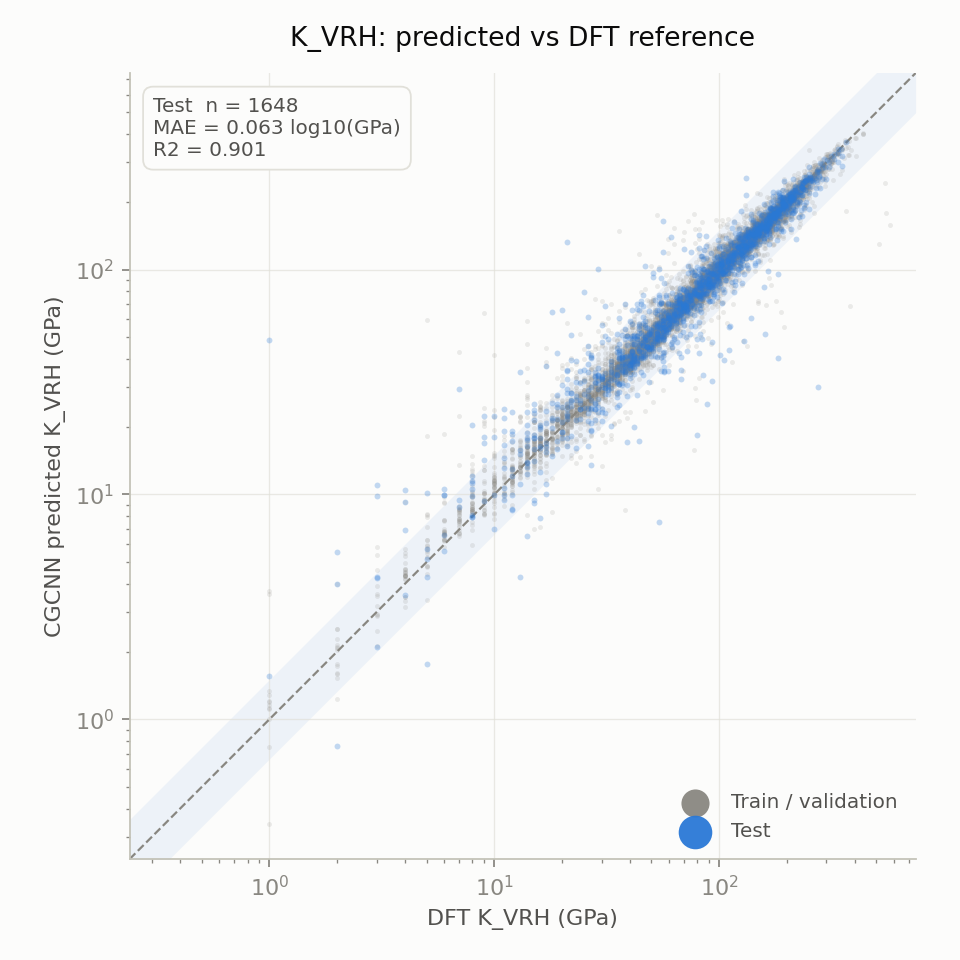
\includegraphics[width=0.82\linewidth]{../results/cgcnn/parity_K_VRH_ens.png}
\end{center}
\column{0.49\linewidth}
\begin{center}
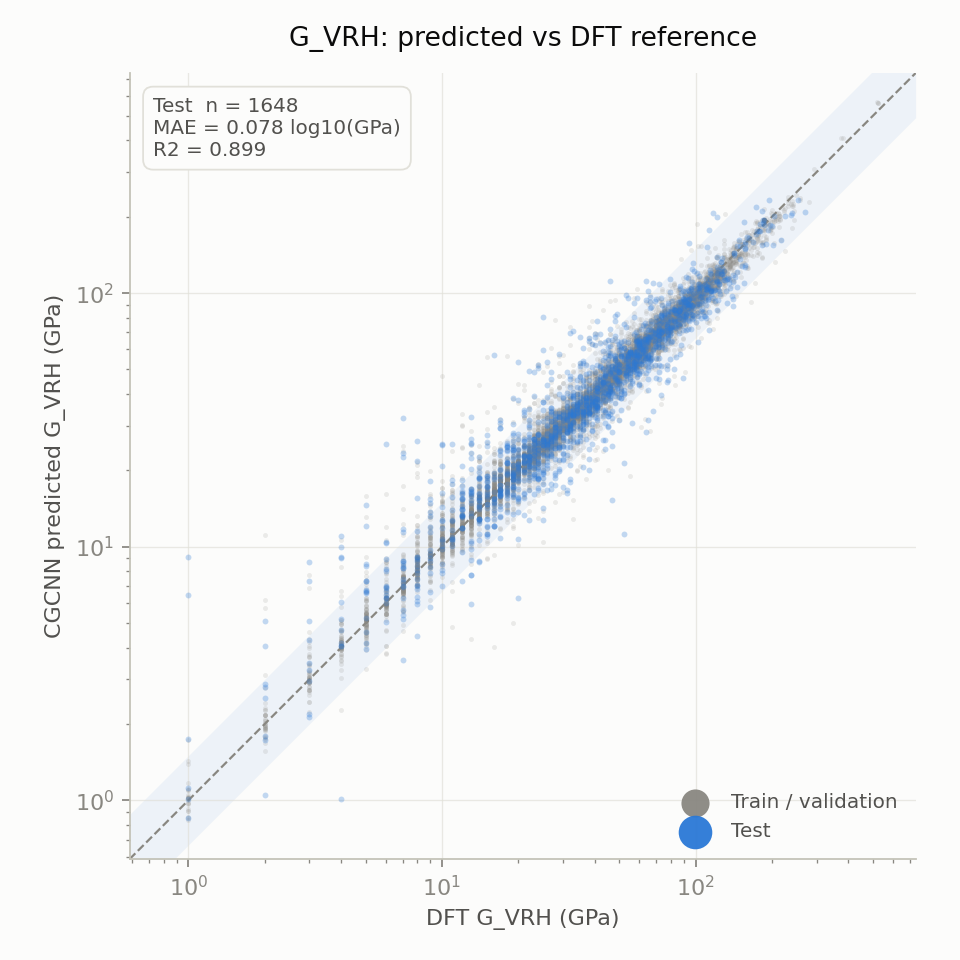
\includegraphics[width=0.82\linewidth]{../results/cgcnn/parity_G_VRH_ens.png}
\end{center}
\end{columns}

\vspace{2pt}
{\sffamily\footnotesize
3-model ensemble, 1{,}648 held-out crystals. Bulk $\KEnsMae$, shear
$\GEnsMae$ MAE $\log_{10}$.}
\end{frame}

% -----------------------------------------------------------------------------
% OLD PAGE 19: Predicted vs DFT - the ALIGNN arm
% now feeds new slide(s): 12
% -----------------------------------------------------------------------------
\begin{frame}
\SlideHeader{11 \textperiodcentered\ RESULTS}{Predicted vs DFT --- the ALIGNN arm}

\begin{columns}[T]
\column{0.49\linewidth}
\begin{center}
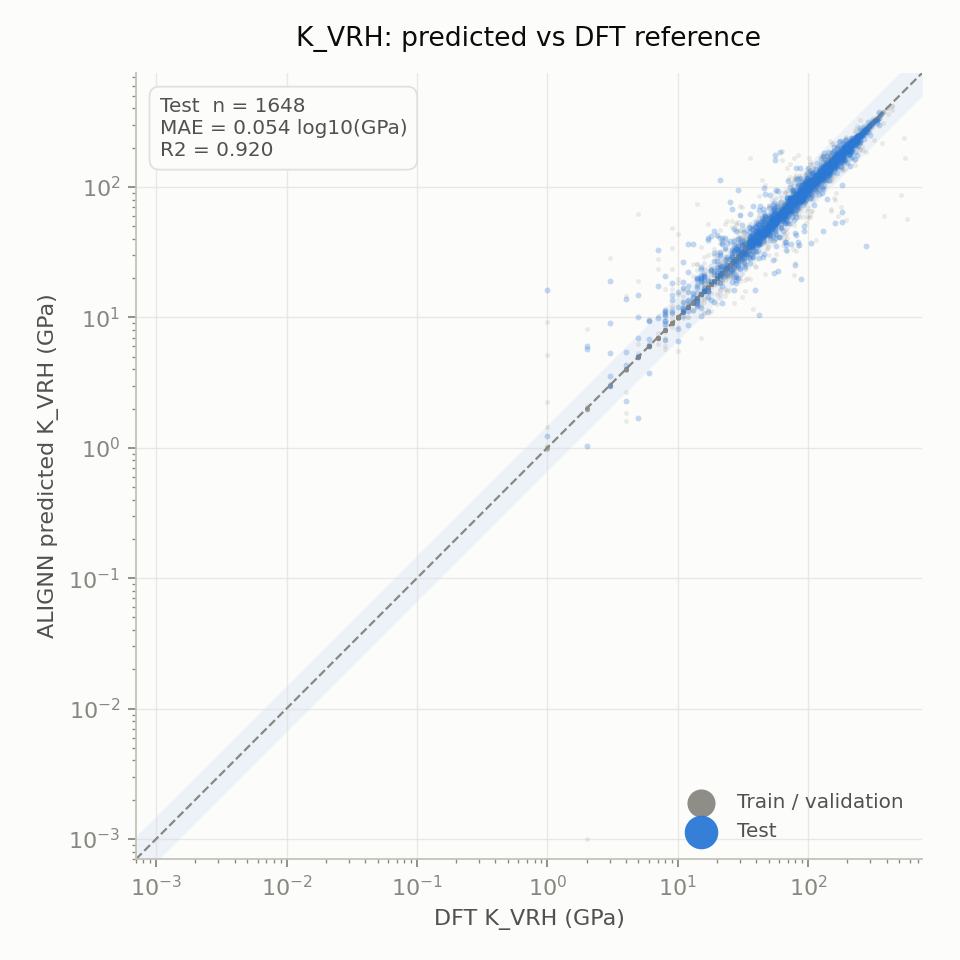
\includegraphics[width=0.80\linewidth]{../results/alignn/parity_K_VRH_alignn.png}
\end{center}
\column{0.49\linewidth}
\begin{center}
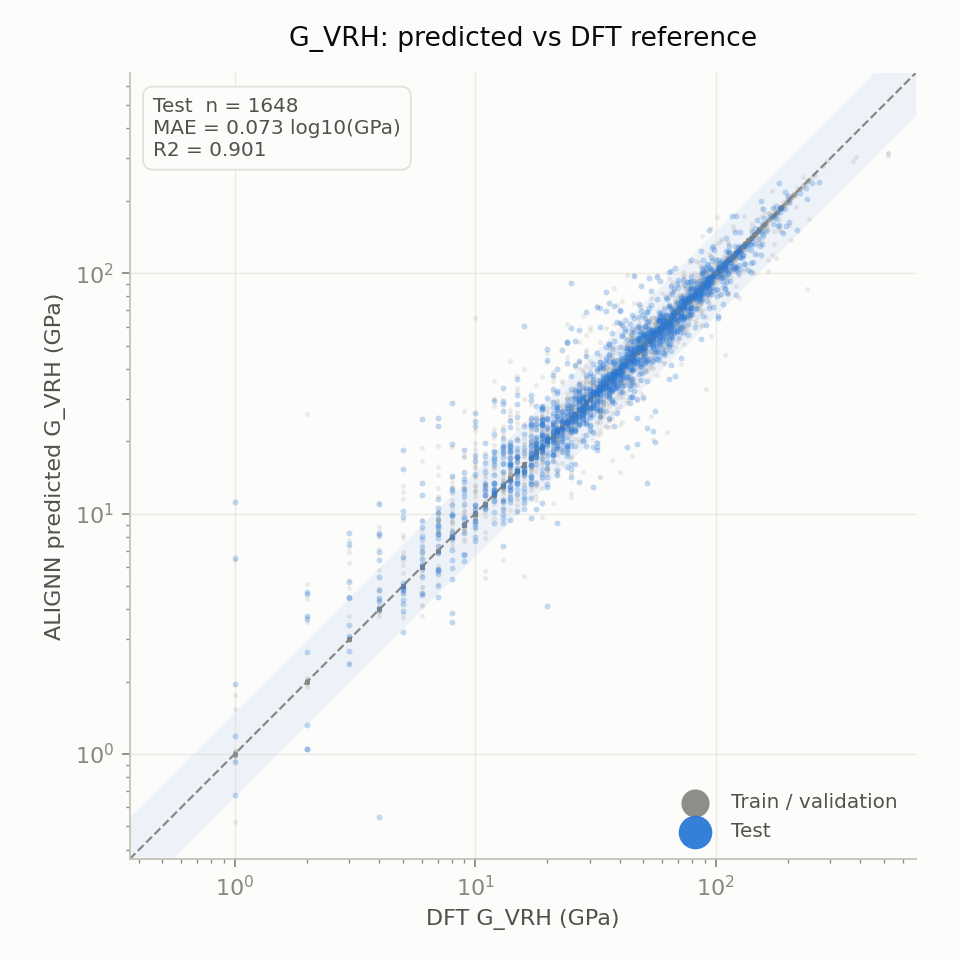
\includegraphics[width=0.80\linewidth]{../results/alignn/parity_G_VRH_alignn.png}
\end{center}
\end{columns}

\vspace{2pt}
{\sffamily\footnotesize
Same crystals and axes. Bulk 0.0539 ($R^2 = 0.920$), shear 0.0725
($R^2 = 0.901$). \textbf{Artefact left visible:} one \emph{negative} bulk
modulus, which a log-space model cannot produce.}
\end{frame}

% -----------------------------------------------------------------------------
% OLD PAGE 20: Where the models fail - residuals
% now feeds new slide(s): 13
% -----------------------------------------------------------------------------
\begin{frame}
\SlideHeader{12 \textperiodcentered\ RESULTS}{Where the models fail --- residuals}

\begin{columns}[T]
\column{0.49\linewidth}
\begin{center}
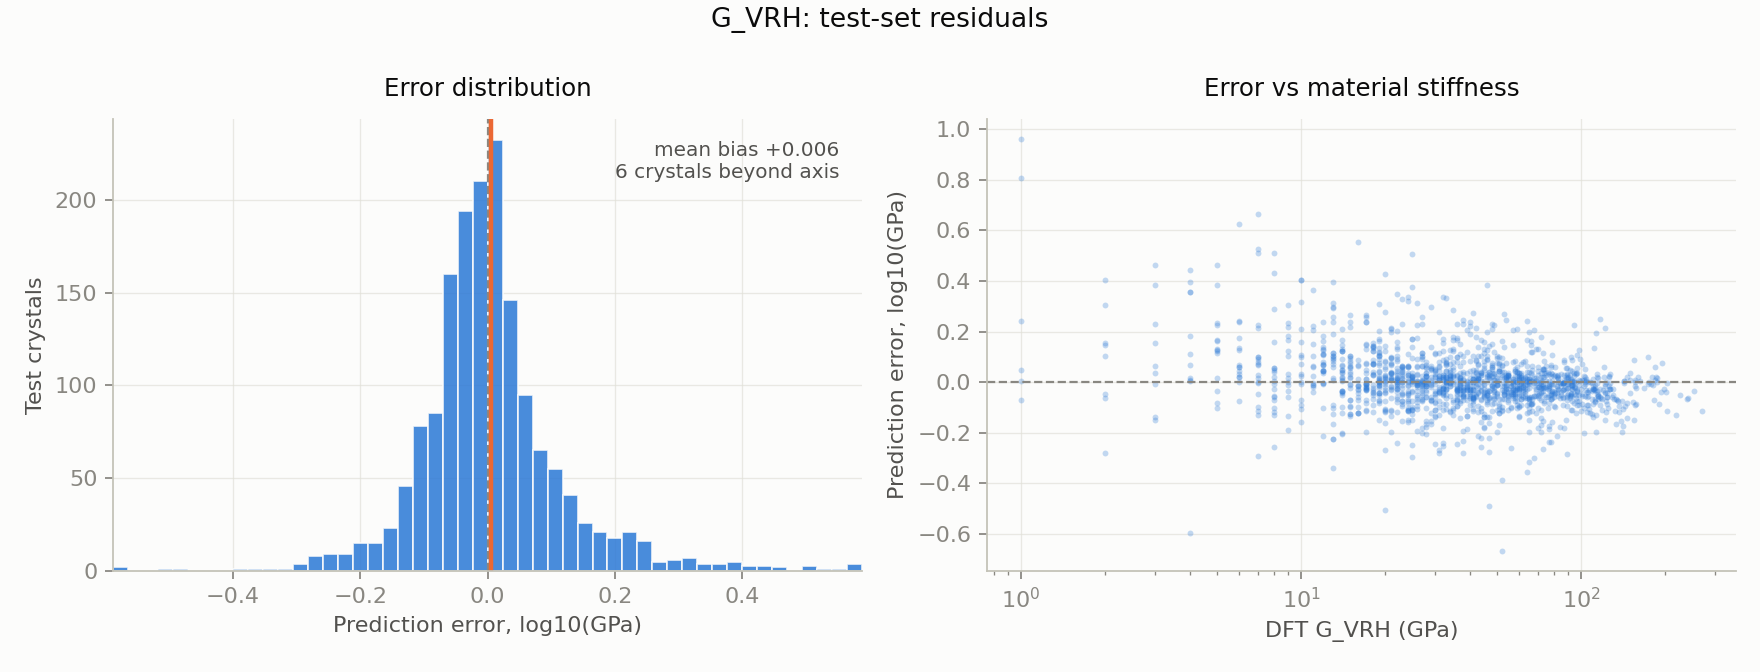
\includegraphics[width=\linewidth]{../results/cgcnn/residuals_G_VRH_ens.png}
\end{center}
{\sffamily\scriptsize\color{Muted}\centering CGCNN ensemble, shear}
\column{0.49\linewidth}
\begin{center}
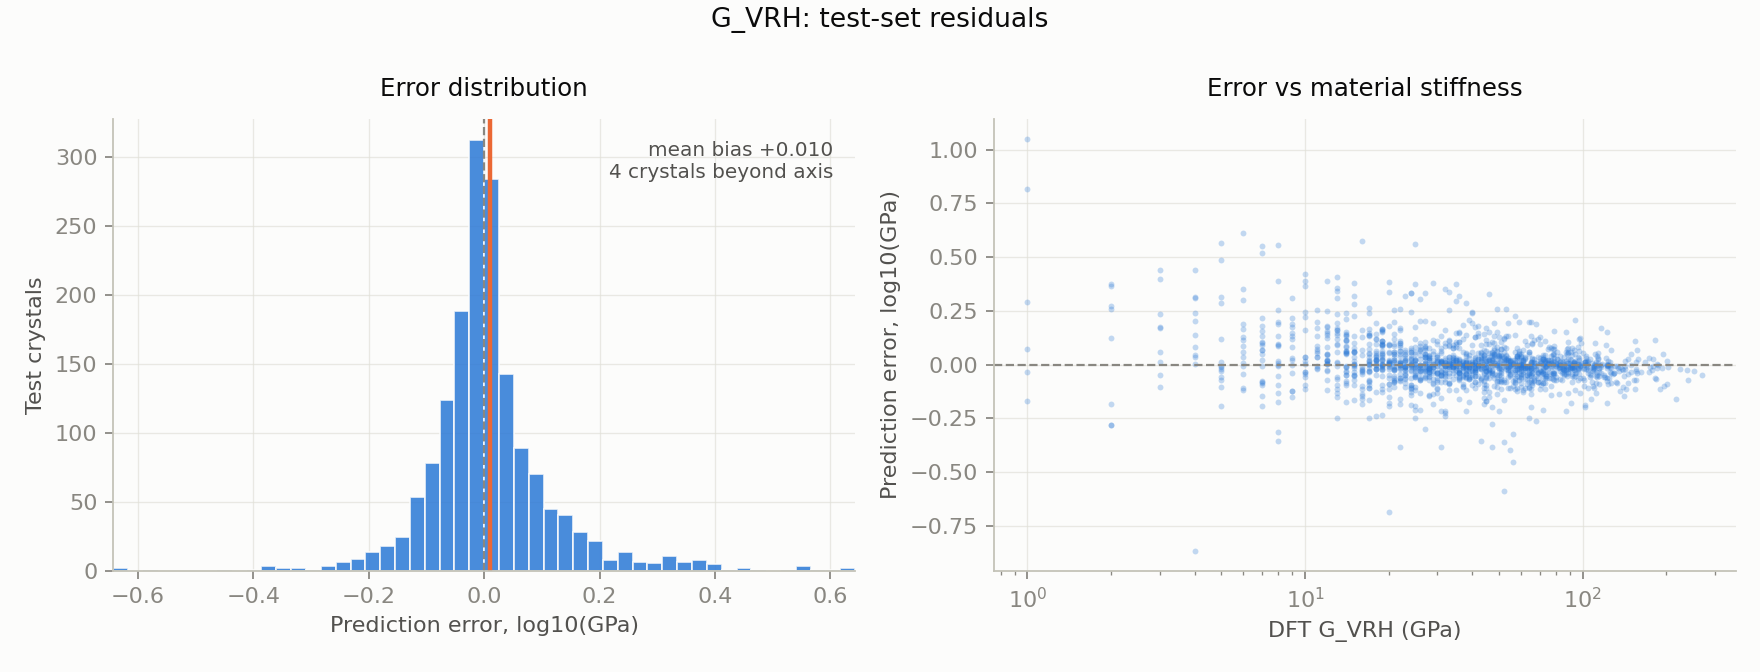
\includegraphics[width=\linewidth]{../results/alignn/residuals_G_VRH_alignn.png}
\end{center}
{\sffamily\scriptsize\color{Muted}\centering ALIGNN, shear}
\end{columns}

\vspace{3pt}
{\sffamily\footnotesize
Residuals fan out below $\sim$30 GPa in both. Stratified by true $\kappa_L$, the
softest quartile has MAE $\log_{10}(G) = 0.134$ against $0.057$ for the
stiffest --- a factor of $2.4$.}

\Takeaway{Both architectures are worst in exactly the regime the screen targets.
Part 7 asks whether that is the model or the labels.}
\end{frame}

% -----------------------------------------------------------------------------
% OLD PAGE 23: What ensembling buys
% now feeds new slide(s): 14
% -----------------------------------------------------------------------------
\begin{frame}
\SlideHeader{13 \textperiodcentered\ RESULTS}{What ensembling buys}

\begin{columns}[T]
\column{0.52\linewidth}
\begin{center}
\includegraphics[width=\linewidth]{figures/ensemble.png}
\end{center}
\column{0.44\linewidth}
{\sffamily\footnotesize
Three models per target, different random initialisations, averaged in
$\log_{10}$ space --- a geometric mean, which is the right notion of middle for
a quantity whose error is proportional.

\vspace{4pt}
Ensembling removed 9--10\% of the error: bulk $\KOneMae \rightarrow \KEnsMae$,
shear $\GOneMae \rightarrow \GEnsMae$.}

\vspace{5pt}
\Card{5.2cm}{CardBg}{CardRule}{%
  \sffamily\footnotesize
  \textbf{And a free uncertainty estimate}\\[3pt]
  The spread across members gives a per-crystal error bar --- the thing PINK's
  single pretrained model cannot produce at all.\\[3pt]
  {\color{SlideAmber}Part 4 shows that estimate is badly overconfident.}}
\end{columns}
\end{frame}

% -----------------------------------------------------------------------------
% OLD PAGE 25: Equations 1--3 - from moduli to sound
% now feeds new slide(s): 15
% -----------------------------------------------------------------------------
\begin{frame}
\SlideHeader{13b \textperiodcentered\ PHYSICS}{Equations 1--3 --- from moduli to sound}

{\sffamily\scriptsize
The two predicted moduli fix how fast sound travels, and phonon speed sets
thermal conductivity.}

\vspace{3pt}
\begin{align}
v_l &= \sqrt{\frac{K + \tfrac{4}{3}G}{\rho}} &&\text{longitudinal wave speed} \\[2pt]
v_t &= \sqrt{\frac{G}{\rho}} &&\text{transverse wave speed} \\[2pt]
v_s &= \left[\frac{1}{3}\left(\frac{1}{v_l^{3}} + \frac{2}{v_t^{3}}\right)\right]^{-1/3}
   &&\text{averaged sound velocity}
\end{align}

\vspace{2pt}
\begin{center}
{\sffamily\scriptsize
\begin{tabular}{@{}lll@{}}
\toprule
sym & meaning & unit \\
\midrule
$K$, $G$ & bulk, shear modulus \emph{(predicted)} & GPa \\
$\rho$ & mass density \emph{(from the CIF)} & g\,cm$^{-3}$ \\
$v_l, v_t, v_s$ & sound velocities & m\,s$^{-1}$ \\
\bottomrule
\end{tabular}}
\end{center}


\end{frame}

% -----------------------------------------------------------------------------
% OLD PAGE 26: Equations 4--6 - Debye temperature and Grüneisen
% now feeds new slide(s): 15
% -----------------------------------------------------------------------------
\begin{frame}
\SlideHeader{13c \textperiodcentered\ PHYSICS}{Equations 4--6 --- Debye temperature and Gr\"uneisen}

\begin{align}
\Theta_D &= \frac{h}{k_B}\left(\frac{3}{4\pi V}\right)^{1/3} v_s
   &&\text{Debye temperature} \\[2pt]
\nu &= \frac{(v_l/v_t)^2 - 2}{2\,(v_l/v_t)^2 - 2} &&\text{Poisson's ratio} \\[2pt]
\gamma &= \frac{3\,(1 + \nu)}{2\,(2 - 3\nu)} &&\text{Gr\"uneisen parameter}
\end{align}

\vspace{2pt}
\begin{center}
{\sffamily\scriptsize
\begin{tabular}{@{}llllll@{}}
\toprule
sym & meaning & unit & sym & meaning & unit \\
\midrule
$h$ & Planck const. & J\,s & $\Theta_D$ & Debye temp. & K \\
$k_B$ & Boltzmann const. & J\,K$^{-1}$ & $\nu$ & Poisson's ratio & --- \\
$V$ & vol.\ per atom \emph{(CIF)} & \AA$^3$ & $\gamma$ & Gr\"uneisen & --- \\
\bottomrule
\end{tabular}}
\end{center}

\vspace{1pt}
{\sffamily\scriptsize
\textbf{Eq.~6 matters most:} $\gamma$ is \emph{derived} from the same $K$, $G$.}
\end{frame}

% -----------------------------------------------------------------------------
% OLD PAGE 27: Equations 7--8 - two routes to $\kappa_L$
% now feeds new slide(s): 16
% -----------------------------------------------------------------------------
\begin{frame}
\SlideHeader{13d \textperiodcentered\ PHYSICS}{Equations 7--8 --- two routes to \texorpdfstring{$\kappa_L$}{kappa}}

\begin{align}
\kappa_L^{\text{Slack}} &=
  \frac{A(\gamma)\,\bar{M}\,V^{1/3}\,\Theta_D^{3}}{\gamma^{2}\,T\,N},
  \qquad A(\gamma) = \frac{2.43\times10^{-8}}{1 - \dfrac{0.514}{\gamma} + \dfrac{0.228}{\gamma^{2}}} \\[3pt]
\kappa_L^{\text{cal}} &= \frac{G\,v_s\,V^{1/3}}{N\,T}\;e^{-\gamma}
  \qquad\text{\sffamily\scriptsize (the boxed equation in the paper's Figure 1)}
\end{align}

\vspace{1pt}
\begin{center}
{\sffamily\scriptsize
\begin{tabular}{@{}llllll@{}}
\toprule
sym & meaning & unit & sym & meaning & unit \\
\midrule
$\bar{M}$ & mean atomic mass & amu & $T$ & temperature, 300 & K \\
$N$ & atoms per cell & --- & $\kappa_L$ & conductivity & W\,m$^{-1}$K$^{-1}$ \\
\bottomrule
\end{tabular}}
\end{center}

\vspace{1pt}
{\sffamily\scriptsize
\textbf{This project reports $\kappa_L^{\text{cal}}$}, whose $\gamma$ dependence
is \emph{exponential}, not $\gamma^{-2}$ --- so swapping $\gamma$ rescales it by
$e^{\gamma_{\text{old}} - \gamma_{\text{new}}}$.}
\end{frame}

% -----------------------------------------------------------------------------
% OLD PAGE 28: The Slack chain - no free parameters
% now feeds new slide(s): 16
% -----------------------------------------------------------------------------
\begin{frame}
\SlideHeader{14 \textperiodcentered\ PHYSICS}{The Slack chain --- no free parameters}

\begin{center}
\scalebox{0.685}{%
\begin{tikzpicture}[node distance=4mm,
  box/.style={rounded corners=4pt, fill=CardBg, draw=CardRule, line width=0.7pt,
              text width=2.45cm, align=center, inner sep=5pt,
              font=\sffamily\scriptsize\color{SlideInk}},
  arr/.style={font=\color{SlideBlue}\small}]
  \node[box] (b1) {$K$, $G$\\ {\color{Muted}predicted}};
  \node[arr, right=of b1] (a1) {$\rightarrow$};
  \node[box, right=of a1] (b2) {Poisson ratio $\nu$};
  \node[arr, right=of b2] (a2) {$\rightarrow$};
  \node[box, right=of a2] (b3) {sound velocities\\ $v_l$, $v_t$, $v_s$};
  \node[arr, right=of b3] (a3) {$\rightarrow$};
  \node[box, right=of a3] (b4) {Debye temp.\\ $\Theta_D$};
  \node[arr, right=of b4] (a4) {$\rightarrow$};
  \node[box, right=of a4] (b5) {$\kappa_L$};
  \node[box, below=8mm of b3, fill=AmberBg, draw=AmberRule] (g)
       {Gr\"uneisen $\gamma$ \\ {\color{Muted}from $\nu$}};
  \draw[->, SlideAmber, line width=0.7pt] (g) -- (b5.south west);
\end{tikzpicture}}
\end{center}

\vspace{2pt}
{\sffamily\footnotesize
Every arrow is a closed-form relation. The only learned quantities in the whole
chain are $K$ and $G$; everything downstream is algebra plus the structural
constants (volume, density, atom count) read straight from the CIF.

\vspace{4pt}
$\gamma$ is \textbf{derived} from the predicted $K/G$ ratio through an empirical
Poisson relation --- matbench contains no measured $\gamma$ at all. That single
choice turns out to dominate several later results.}

\Takeaway{Because the physics is shared and unchanged, any difference between
two of this project's screens is the \emph{moduli}, never the formula.}
\end{frame}

% -----------------------------------------------------------------------------
% OLD PAGE 29: The uncertainty interval was badly overconfident
% now feeds new slide(s): 17
% -----------------------------------------------------------------------------
\begin{frame}
\SlideHeader{15 \textperiodcentered\ PHYSICS}{The uncertainty interval was badly overconfident}

\begin{columns}[T]
\column{0.52\linewidth}
\begin{center}
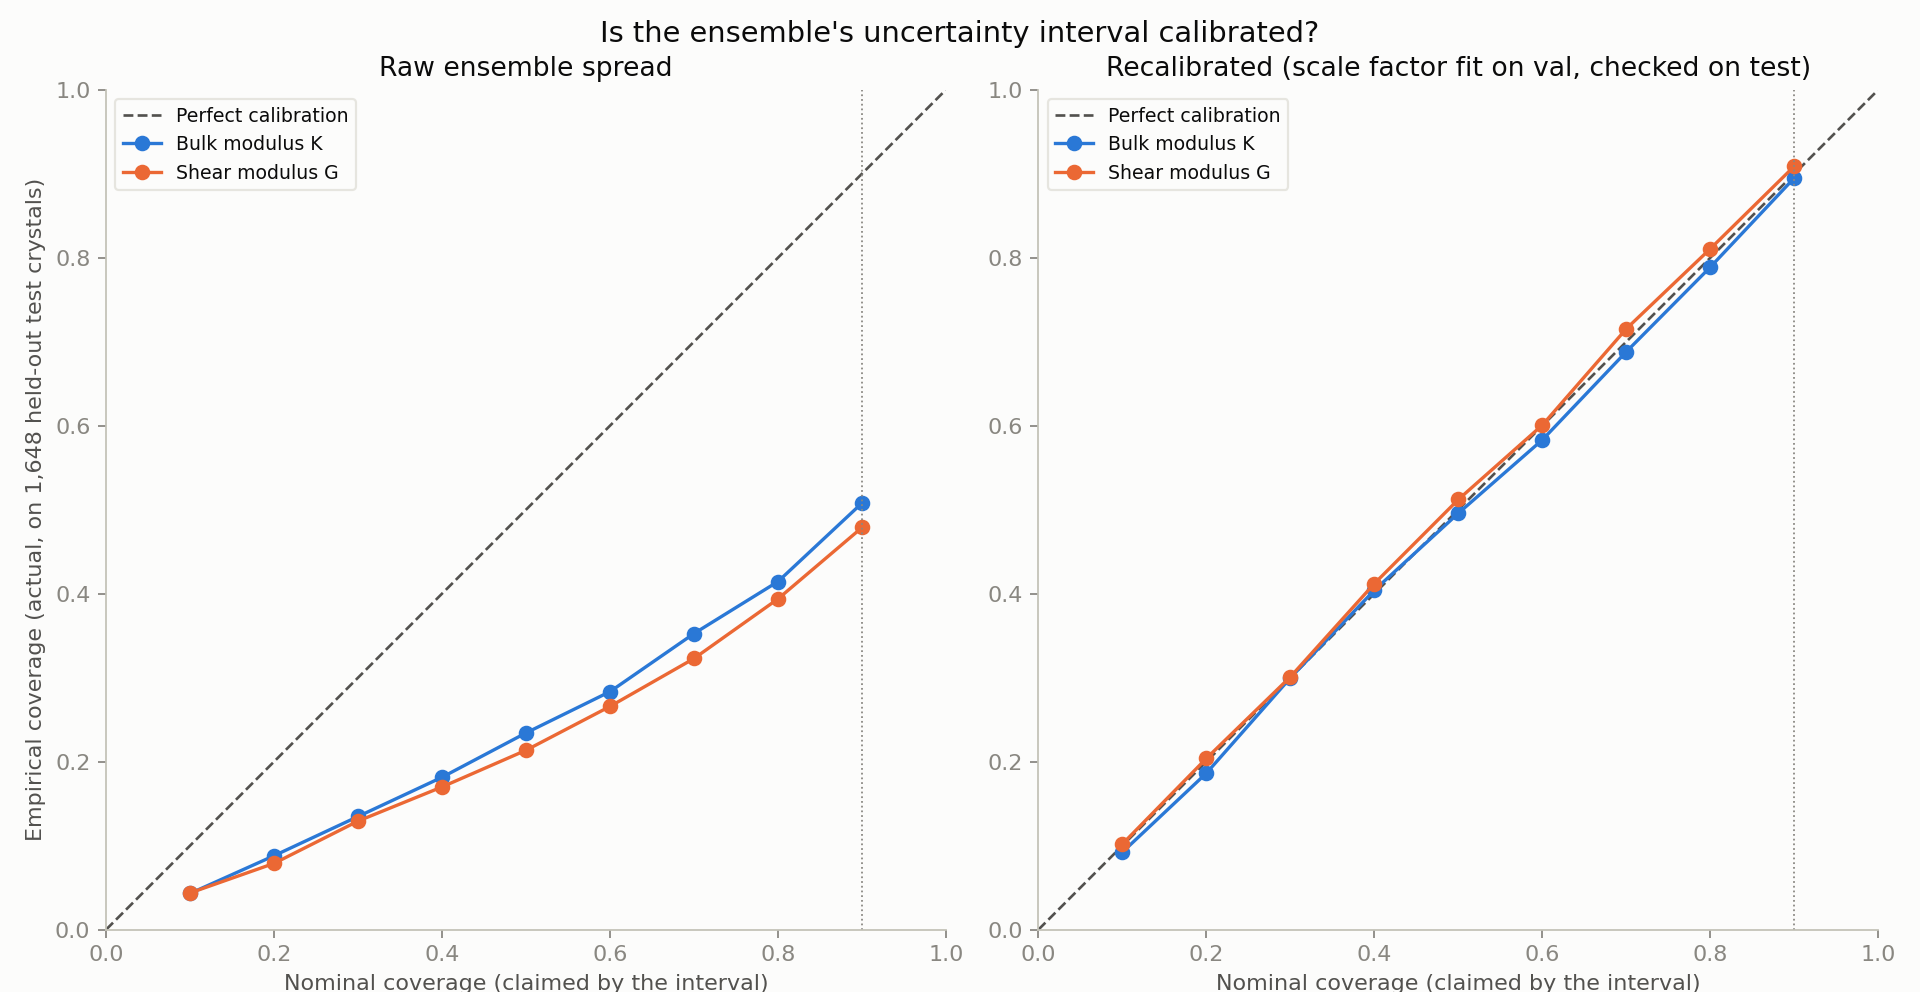
\includegraphics[width=\linewidth]{../results/cgcnn/calibration_check.png}
\end{center}
\column{0.44\linewidth}
{\sffamily\footnotesize
The Monte Carlo p05--p95 band was checked against the test split's real DFT
labels --- no new data needed.}

\vspace{5pt}
\AccentCard{5.2cm}{SlideAmber}{%
  \sffamily\footnotesize
  \textbf{Claimed 90\% coverage. Actual 48--51\%.}\\[3pt]
  Cause: three identically-trained members share blind spots, so member
  \emph{disagreement} runs 4--6$\times$ smaller than true error.}

\vspace{4pt}
{\sffamily\scriptsize
Recalibration factors from validation ($K$ 4.27$\times$, $G$ 4.54$\times$)
recover $\sim$90\% coverage out of sample --- and collapse almost every
``tight'' label on the DFT shortlist to ``wide''.}
\end{columns}

\Takeaway{An ensemble's spread measures variance. The error is bias plus
variance --- and here bias dominates.}
\end{frame}

% -----------------------------------------------------------------------------
% OLD PAGE 31: Measured $\kappa_L$ - PINK's Figure 6B, our version
% now feeds new slide(s): 18
% -----------------------------------------------------------------------------
\begin{frame}
\SlideHeader{16 \textperiodcentered\ REAL DATA}{Measured $\kappa_L$ --- PINK's Figure 6B, our version}

\begin{columns}[T]
\column{0.55\linewidth}
\begin{center}
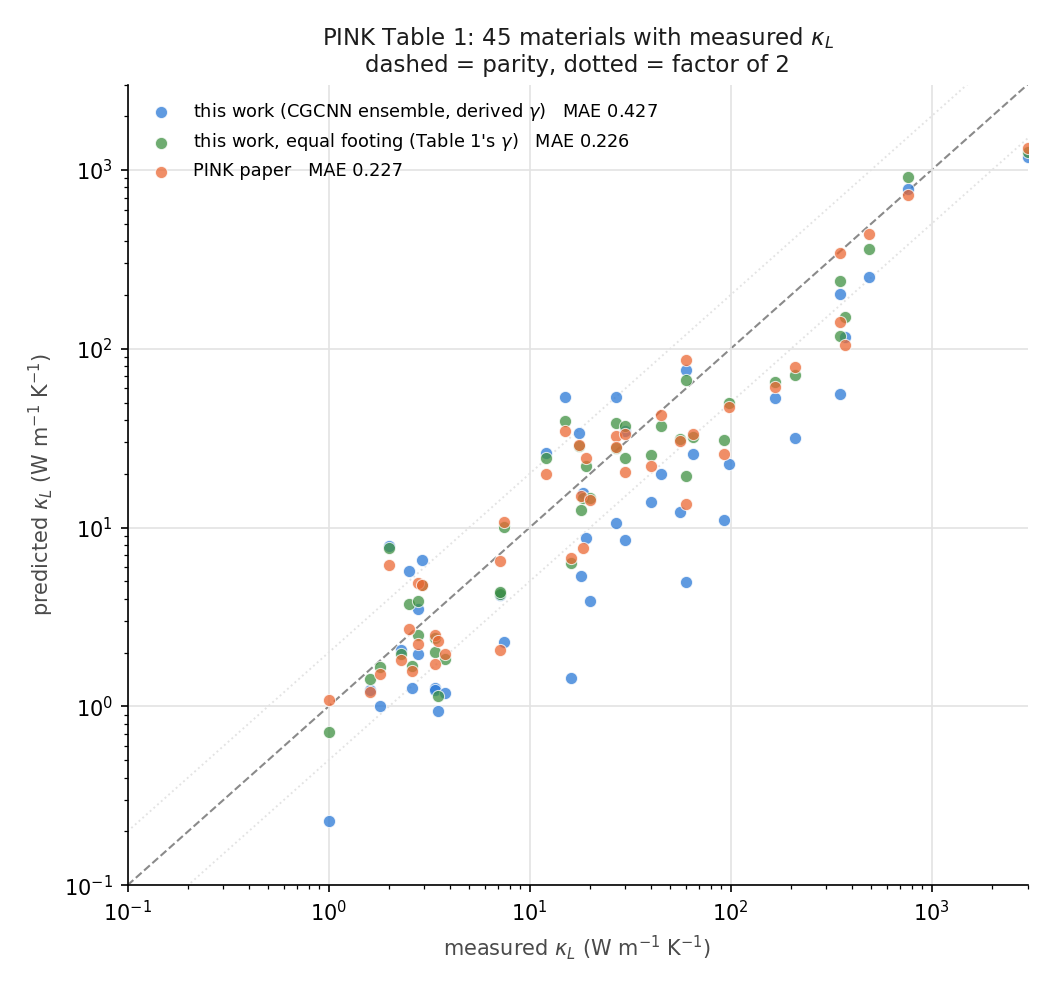
\includegraphics[width=0.72\linewidth]{../results/cgcnn/63_experimental_vs_predicted.png}
\end{center}
\column{0.41\linewidth}
{\sffamily\footnotesize
The paper's Table 1 lists 46 materials with \textbf{experimentally measured}
$\kappa_L$. 45 survive (mp-3490/GaP is deprecated in Materials Project).

\vspace{4pt}
The range spans four orders of magnitude --- AgCl at 1.0 to diamond at 3000
W\,m$^{-1}$K$^{-1}$ --- so everything is scored in $\log_{10}$.}

\vspace{5pt}
\Card{5.0cm}{CardBg}{CardRule}{%
  \sffamily\scriptsize
  \textbf{mean $|\Delta \log_{10}|$}\\[3pt]
  ours, derived $\gamma$ \dotfill 0.427\\
  ours, equal footing \dotfill \textbf{0.226}\\
  the PINK paper \dotfill 0.227}
\end{columns}

\Takeaway{At face value we look twice as bad; on equal footing we match it.}
\end{frame}

% -----------------------------------------------------------------------------
% OLD PAGE 32: The comparison was never like-for-like
% now feeds new slide(s): 18
% -----------------------------------------------------------------------------
\begin{frame}
\SlideHeader{17 \textperiodcentered\ REAL DATA}{The comparison was never like-for-like}

\begin{columns}[T]
\column{0.46\linewidth}
{\sffamily\footnotesize
Table 1's $\gamma$ values come from \textbf{AFLOW / experimental lookups} ---
the paper's own text says so. They are \emph{not} produced by the Poisson-ratio
formula that our pipeline uses.

\vspace{4pt}
Neither does the paper's own released screening code use them: it uses the same
formula we do. So comparing our derived $\gamma$ against a looked-up-$\gamma$
table tests \textbf{the $\gamma$ source}, not the model.}

\vspace{5pt}
\Card{5.6cm}{CardBg}{CardRule}{%
  \sffamily\footnotesize
  \textbf{Substituting Table 1's own $\gamma$}\\[3pt]
  changes nothing else --- same moduli, same physics ---\\[2pt]
  $0.427 \rightarrow \mathbf{0.226}$\\[2pt]
  against the paper's $0.227$.}

\column{0.50\linewidth}
\begin{center}
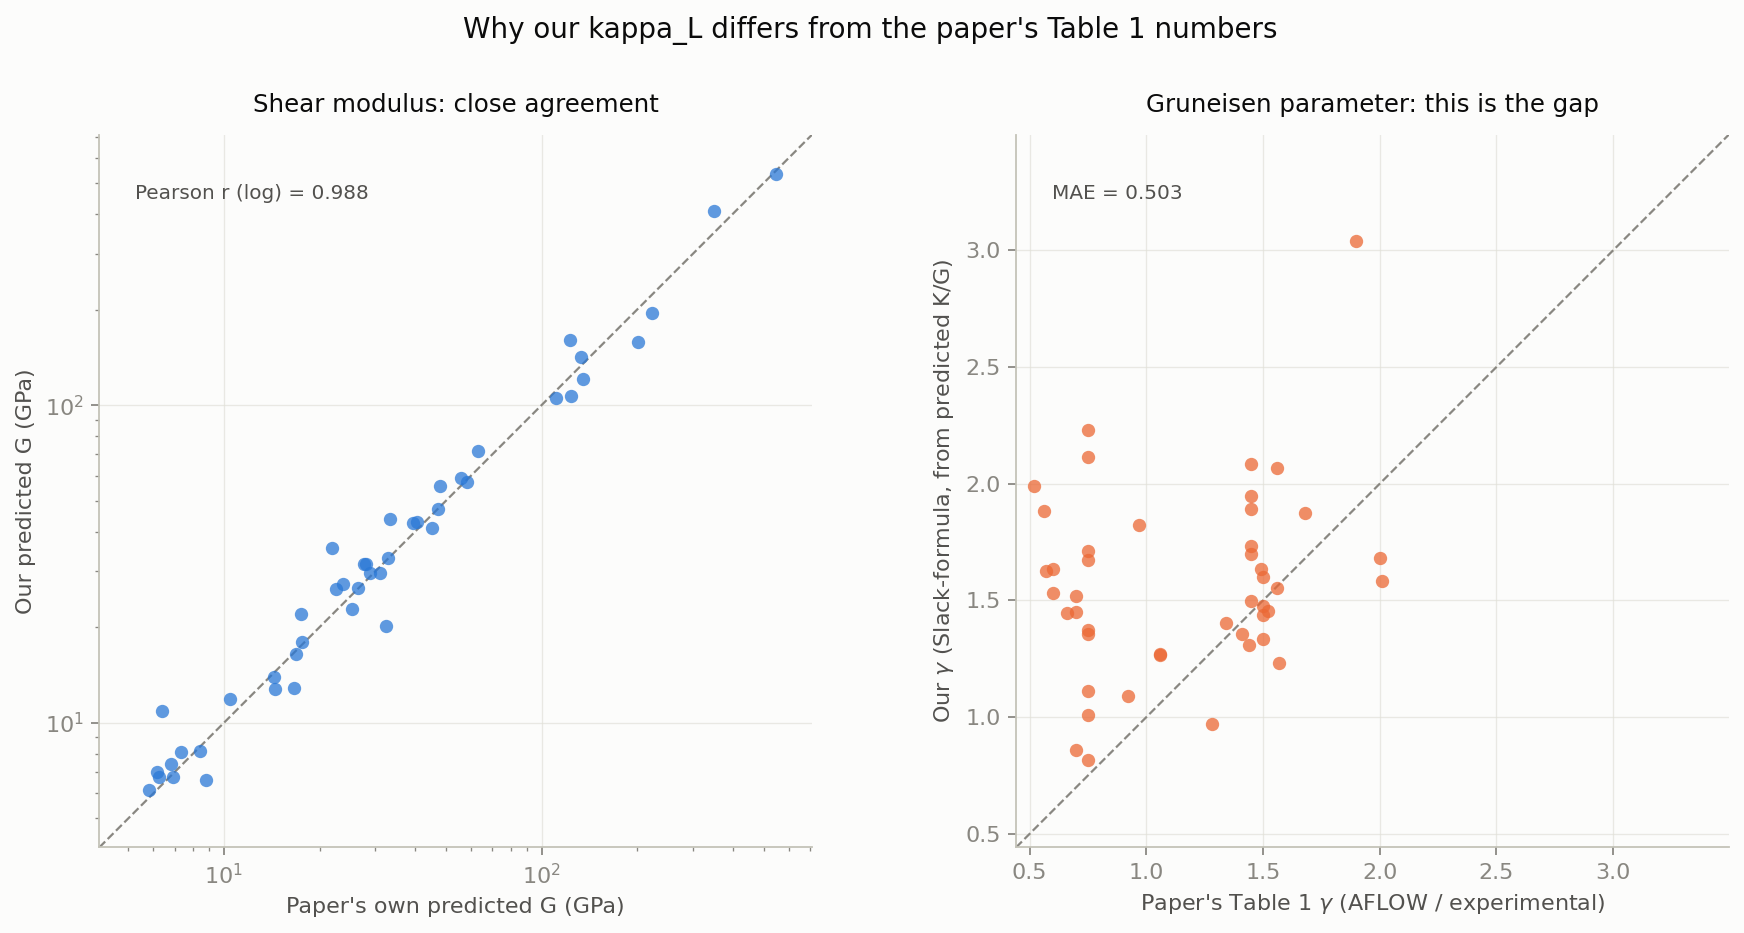
\includegraphics[width=\linewidth]{../results/cgcnn/table1_gamma_diagnostic.png}
\end{center}
{\sffamily\scriptsize\color{Muted}\centering
Our moduli were never the problem: shear modulus and sound velocity agree with
the paper's own tabulated values at $r \approx 0.99$.}
\end{columns}

\Takeaway{The paper does not state this; it took investigation to find.}
\end{frame}

% -----------------------------------------------------------------------------
% OLD PAGE 34: Two architectures, independently, on the same 1,213 crystals
% now feeds new slide(s): 19
% -----------------------------------------------------------------------------
\begin{frame}
\SlideHeader{19 \textperiodcentered\ REAL DATA}{Two architectures, independently, on the same 1{,}213 crystals}

\begin{columns}[T]
\column{0.52\linewidth}
\begin{center}
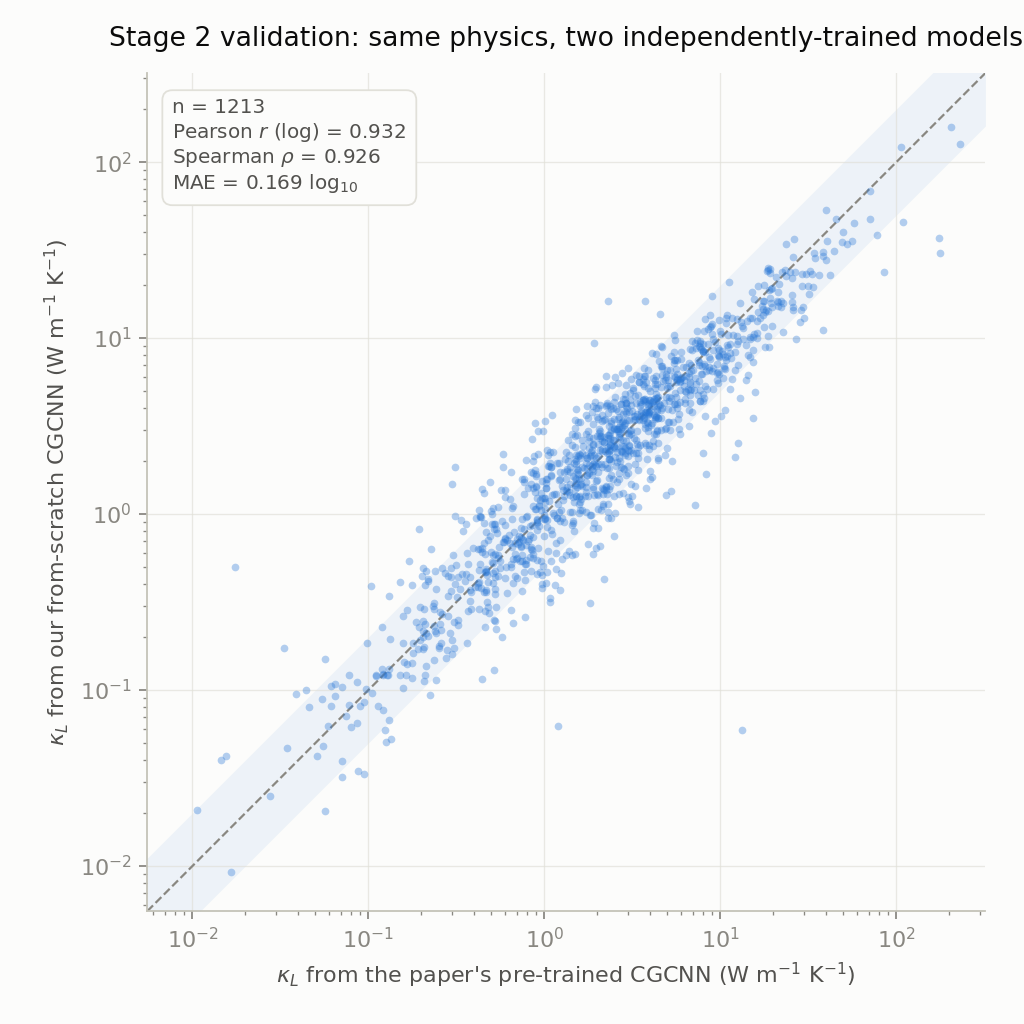
\includegraphics[width=0.74\linewidth]{../results/cgcnn/kappa_validation.png}
\end{center}
\column{0.44\linewidth}
{\sffamily\footnotesize
ALIGNN's moduli pushed through the \emph{unchanged} Slack chain, compared
against the CGCNN ensemble's $\kappa_L$ on the same crystals.

\vspace{4pt}
\textbf{Pearson $r = 0.940$, Spearman $\rho = 0.947$}, MAE 0.141 $\log_{10}$ ---
tighter than CGCNN's own agreement with the paper's pretrained model
($r = 0.932$).}

\vspace{5pt}
\Card{5.2cm}{CardBg}{CardRule}{%
  \sffamily\footnotesize
  Two independently trained architectures, sharing only the data, the split and
  the physics, converging this closely on final $\kappa_L$ is evidence the
  pipeline finds physical signal.}
\end{columns}
\end{frame}

% -----------------------------------------------------------------------------
% OLD PAGE 36: The screening funnel - PINK's Figure 7
% now feeds new slide(s): 21
% -----------------------------------------------------------------------------
\begin{frame}
\SlideHeader{20 \textperiodcentered\ THE SCREEN}{The screening funnel --- PINK's Figure 7}

\begin{center}
\begin{tikzpicture}[node distance=4mm,
  box/.style={rounded corners=4pt, fill=CardBg, draw=CardRule, line width=0.7pt,
              text width=3.0cm, align=center, inner sep=6pt,
              font=\sffamily\scriptsize\color{SlideInk}},
  hit/.style={rounded corners=4pt, fill=GreenBg, draw=GreenRule, line width=0.8pt,
              text width=3.0cm, align=center, inner sep=6pt,
              font=\sffamily\scriptsize\color{SlideInk}},
  arr/.style={font=\color{SlideBlue}\small}]
  \node[box] (b1) {\textbf{554{,}054}\\ GNoME stable materials};
  \node[arr, right=of b1] (a1) {$\rightarrow$};
  \node[box, right=of a1] (b2) {\textbf{33{,}118}\\ pass the paper's own filters};
  \node[arr, right=of b2] (a2) {$\rightarrow$};
  \node[box, right=of a2] (b3) {score $K$, $G$\\ $\rightarrow$ Slack $\rightarrow \kappa_L$};
  \node[arr, right=of b3] (a3) {$\rightarrow$};
  \node[hit, right=of a3] (b4) {\textbf{$\kappa_L \leq 1$}\\ W\,m$^{-1}$K$^{-1}$};
\end{tikzpicture}
\end{center}

\vspace{4pt}
{\sffamily\footnotesize
The current GNoME snapshot holds \textbf{554{,}054} materials against the
paper's 377{,}221 --- stated explicitly rather than glossed, because it means
the candidate lists are not directly comparable.

\vspace{4pt}
Against the paper's own published 11{,}869 candidates, \textbf{70.8\%} also
appear in our independently derived list. Two pipelines sharing only an
architecture family and a physics formula, on overlapping-but-different
corpora, converging on most of the same discoveries.}

\Takeaway{{\color{SlideAmber}Flagged:} that 70.8\% predates several corrections in
Part 7 and should be recomputed before it is quoted in a paper.}
\end{frame}

% -----------------------------------------------------------------------------
% OLD PAGE 37: What the candidates look like - PINK's Figure 8
% now feeds new slide(s): 22
% -----------------------------------------------------------------------------
\begin{frame}
\SlideHeader{21 \textperiodcentered\ THE SCREEN}{What the candidates look like --- PINK's Figure 8}

\begin{columns}[T]
\column{0.49\linewidth}
\begin{center}
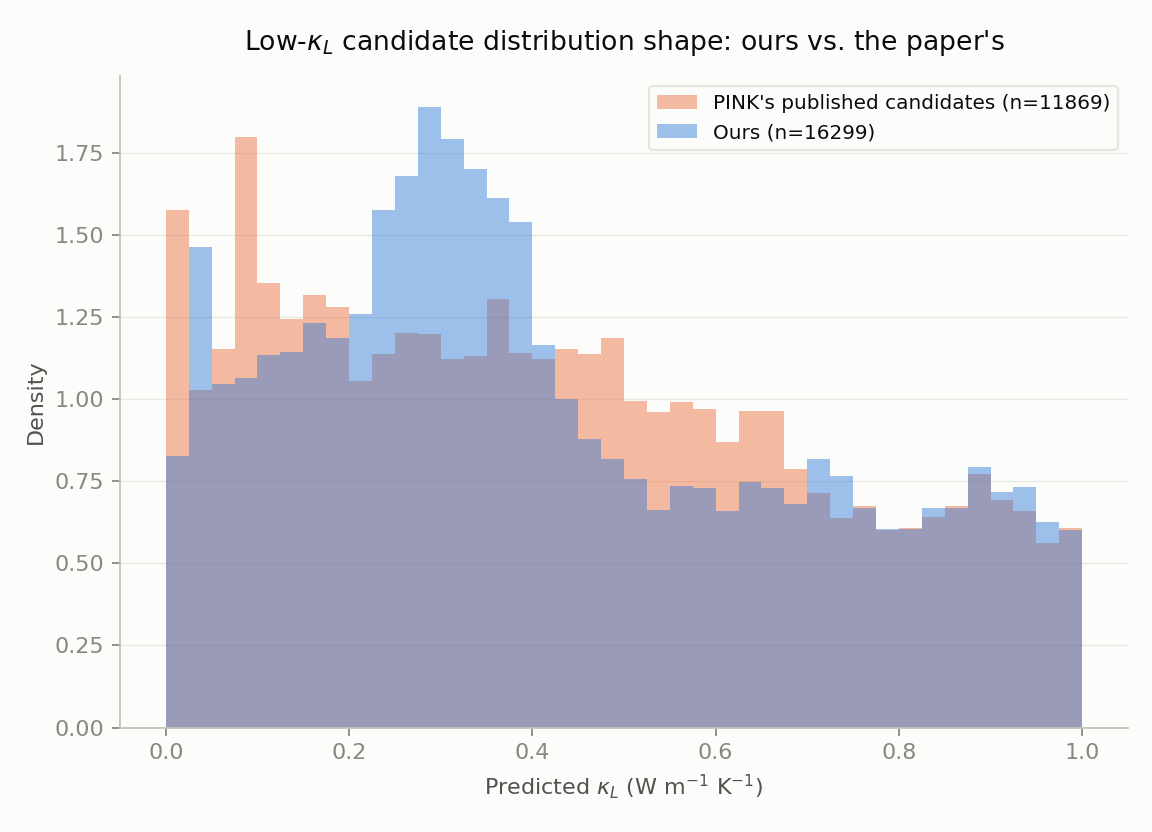
\includegraphics[width=\linewidth]{../results/cgcnn/gnome_kappa_distributions.png}
\end{center}
\column{0.49\linewidth}
\begin{center}
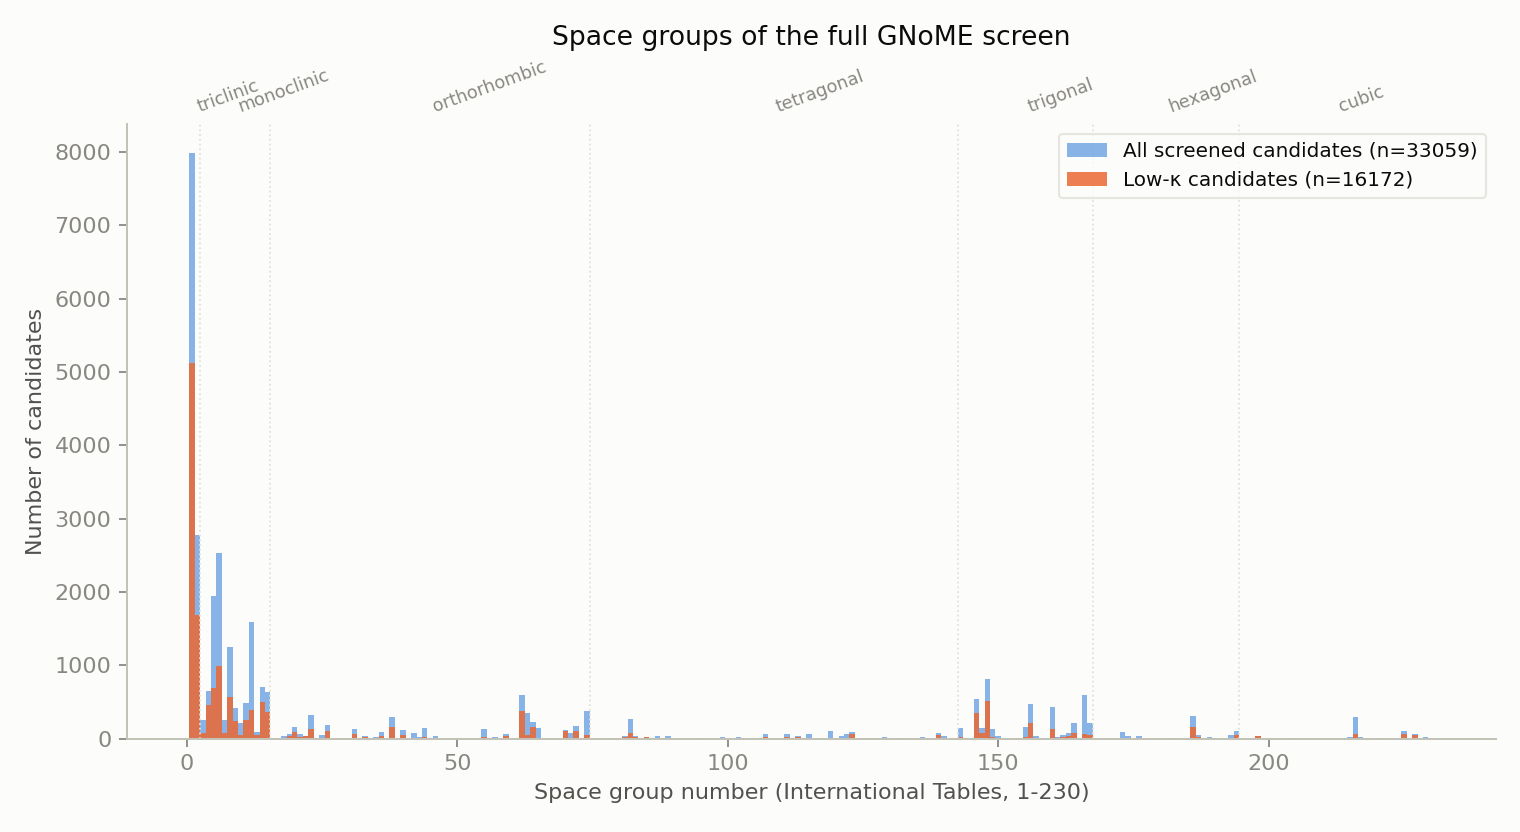
\includegraphics[width=\linewidth]{../results/cgcnn/gnome_screen_spacegroups.png}
\end{center}
\end{columns}

\vspace{2pt}
{\sffamily\scriptsize
$\kappa_L$ distribution and crystal-system breakdown of the screened pool.
Halogens are 1.4--1.9$\times$ enriched among low-$\kappa$ candidates, oxygen
0.27$\times$ depleted.}
\end{frame}

% -----------------------------------------------------------------------------
% OLD PAGE 41: Classifying the candidates: elements
% now feeds new slide(s): 24
% -----------------------------------------------------------------------------
\begin{frame}
\SlideHeader{22c \textperiodcentered\ THE SCREEN}{Classifying the candidates: elements}

\begin{center}
\includegraphics[width=0.86\linewidth]{figures/elements_all_models.png}
\end{center}

\vspace{-3pt}
{\sffamily\scriptsize
Enrichment is how often candidates containing an element are called
low-$\kappa$, over that model's own base rate. Lines are binned medians.
\textbf{Cs, Rb, K and the halogens Br, Cl, F sit high; O and N sit lowest} ---
which Equations 1--3 predict, since a low $G$ gives a low $v_s$. \textbf{All
four agree on the shape}; round 9 diverges at the electronegative end.}
\end{frame}

% -----------------------------------------------------------------------------
% OLD PAGE 51: One file holds every metric of every model
% now feeds new slide(s): 25
% -----------------------------------------------------------------------------
\begin{frame}
\SlideHeader{29 \textperiodcentered\ AUDIT}{One file holds every metric of every model}

{\sffamily\footnotesize
Part 7 found numbers that were wrong, so every metric the project ever stored was
\textbf{recomputed from scratch}. The formulas were re-written, not imported ---
an old bug cannot hide by being re-used.\par}

\vspace{5pt}
\begin{center}
\begin{tikzpicture}[node distance=1.6mm,
  pill/.style={rounded corners=4pt, fill=CardBg, draw=CardRule, line width=0.6pt,
               text width=2.45cm, minimum height=1.45cm, align=center, inner sep=3pt,
               font=\sffamily\scriptsize\color{SlideInk}},
  arr/.style={font=\color{SlideBlue}\normalsize, inner sep=0pt}]
  \node[pill] (p1) {\textbf{1. Inventory}\\ 66 prediction files,\\ 146 stored metric files};
  \node[arr, right=of p1] (a1) {$\rightarrow$};
  \node[pill, right=of a1] (p2) {\textbf{2a. Accuracy}\\ MAE, MSE, $R^2$, $\rho$ from the saved predictions};
  \node[arr, right=of p2] (a2) {$\rightarrow$};
  \node[pill, right=of a2] (p3) {\textbf{2b. Screening}\\ precision, recall, hits, bootstraps from the inputs};
  \node[arr, right=of p3] (a3) {$\rightarrow$};
  \node[pill, right=of a3, draw=SlideBlue] (p4) {\textbf{3. One table}\\ 9{,}740 rows, plus 179 cross-file checks};
\end{tikzpicture}
\end{center}

\vspace{3pt}
\begin{columns}[T]
\column{0.54\linewidth}
{\sffamily\scriptsize
\begin{tabular}{@{}ll@{}}
\toprule
\textbf{column} & \textbf{what it holds} \\
\midrule
\texttt{recomputed} & the number rebuilt now \\
\texttt{stored}     & the number in the old file (\texttt{stored\_in}) \\
\texttt{abs\_diff}  & $|$recomputed $-$ stored$|$ \\
\texttt{rel\_diff}  & abs\_diff $\div$ $|$stored$|$ --- the gap as a fraction \\
\texttt{status}     & the verdict, by the rule on the right \\
\texttt{primary}    & True on the first row of each metric: \\
                    & \quad filter on it to see every number once \\
\bottomrule
\end{tabular}}
\column{0.42\linewidth}
\Card{5.2cm}{CardBg}{CardRule}{%
  \sffamily\scriptsize
  \textbf{The status rule}\\[2pt]
  \textcolor{SlideBlue}{\textbf{match}}: gap $\leq$ half a unit in the stored
  number's last digit (or 1 part in a million)\\[1pt]
  \textcolor{SlideAmber}{\textbf{close}}: gap $\leq$ 0.1\%\\[1pt]
  \textcolor{SlideRed}{\textbf{MISMATCH}}: anything larger\\[1pt]
  \textbf{new}: never saved before (e.g.\ $R^2$ for a run that kept only MAE)\\[1pt]
  \textbf{stored only}: carried over from its file, not rebuilt\par}
\end{columns}
\end{frame}

% -----------------------------------------------------------------------------
% OLD PAGE 52: The verdict: zero mismatches
% now feeds new slide(s): 25
% -----------------------------------------------------------------------------
\begin{frame}
\SlideHeader{30 \textperiodcentered\ AUDIT}{The verdict: zero mismatches}

\begin{center}
\includegraphics[width=0.94\linewidth]{figures/audit_status.png}
\end{center}

\vspace{-2pt}
\begin{columns}[T]
\column{0.31\linewidth}
\AccentCard{3.75cm}{SlideBlue}{%
  \sffamily\scriptsize
  \textbf{4{,}337 rebuilt and identical}\\[2pt]
  Every accuracy and screening number that had been reported, recomputed from
  its inputs and matched.\par}
\column{0.31\linewidth}
\AccentCard{3.75cm}{SlideAmber}{%
  \sffamily\scriptsize
  \textbf{11 close, all below 0.1\%}\\[2pt]
  Models trained on a GPU and re-run on a CPU: the 4th--5th decimal moves. Same
  number, different arithmetic.\par}
\column{0.31\linewidth}
\AccentCard{3.75cm}{SlideGreen}{%
  \sffamily\scriptsize
  \textbf{473 checks, all pass}\\[2pt]
  294 rebuild checks + 179 cross-file ones, e.g.\ each Kaggle summary table
  equals its own JSON files.\par}
\end{columns}

\Takeaway{9{,}048 distinct values, 0 MISMATCH. The 3{,}219 ``new'' values ($R^2$,
MSE, Spearman for runs that only kept MAE) mean every model now has the full set
of metrics, not just the one that was quoted.}
\end{frame}

% -----------------------------------------------------------------------------
% OLD PAGE 53: The moduli models, from that one file
% now feeds new slide(s): 26
% -----------------------------------------------------------------------------
\begin{frame}
\SlideHeader{31 \textperiodcentered\ AUDIT}{The moduli models, from that one file}

\begin{center}
{\sffamily\scriptsize
\begin{tabular}{@{}lrrrrr@{}}
\toprule
& \multicolumn{2}{c}{\textbf{bulk $K$}} & \multicolumn{2}{c}{\textbf{shear $G$}} & \textbf{$\kappa_L$} \\
\cmidrule(lr){2-3}\cmidrule(lr){4-5}\cmidrule(l){6-6}
\textbf{model} & MAE & $R^2$ & MAE & $R^2$ & MAE \\
\midrule
\TableRows{figures/audit_moduli_table.tex}
\bottomrule
\end{tabular}}
\end{center}

\vspace{3pt}
{\sffamily\scriptsize
All on the same 1{,}648 matbench test crystals (\texttt{split\_seed = 42}); MAE
and $R^2$ in $\log_{10}$. The $\kappa_L$ column scores the Slack chain on
\emph{predicted} moduli against the same chain on the \emph{DFT} moduli (the
in-house reference of slide 23), not against a phonon calculation. The trees
never had a $\kappa$ run; the joint model's per-modulus MAE is stored under its
$\kappa$ target and read from there.\par}

\Takeaway{ALIGNN's 3-ensemble is best in every column. Each graph network beats
both composition-only trees on matbench --- a ranking that Part 7 showed
reverses on AFLOW for an underfit network.}
\end{frame}

% -----------------------------------------------------------------------------
% OLD PAGE 54: Against measurement and phonon DFT
% now feeds new slide(s): 20
% -----------------------------------------------------------------------------
\begin{frame}
\SlideHeader{32 \textperiodcentered\ AUDIT}{Against measurement and phonon DFT}

\begin{center}
{\sffamily\scriptsize
\begin{tabular}{@{}llll@{}}
\toprule
\textbf{test set} & \textbf{model} & \textbf{measured as} & \textbf{value} \\
\midrule
\TableRows{figures/audit_truth_table.tex}
\bottomrule
\end{tabular}}
\end{center}

\vspace{2pt}
\begin{columns}[T]
\column{0.31\linewidth}
\AccentCard{3.75cm}{SlideBlue}{%
  \sffamily\scriptsize
  \textbf{Measured $\kappa_L$ (45)}\\[2pt]
  With the paper's own $\gamma$ we match the paper: 0.226 vs 0.227. With $\gamma$
  from Poisson's ratio the error doubles --- $\gamma$, not the network, is the
  weak link.\par}
\column{0.31\linewidth}
\AccentCard{3.75cm}{SlideGreen}{%
  \sffamily\scriptsize
  \textbf{Phonon DFT (2{,}520)}\\[2pt]
  3 in 4 crystals the chain calls $\leq 1$ really are. Swapping in a phonon
  $\gamma$ from an MLIP adds +0.013 --- its interval spans zero, so no
  measurable gain.\par}
\column{0.31\linewidth}
\AccentCard{3.75cm}{SlideAmber}{%
  \sffamily\scriptsize
  \textbf{Direct ALIGNN}\\[2pt]
  Trained straight on phonon-DFT $\kappa_L$, no Slack formula. Each crystal
  predicted once, while held out: typical miss $\times$1.56 ($10^{0.194}$),
  rank $\rho = 0.89$.\par}
\end{columns}
\end{frame}

% -----------------------------------------------------------------------------
% OLD PAGE 57: From 554,054 materials to 15 crystals
% now feeds new slide(s): 27
% -----------------------------------------------------------------------------
\begin{frame}
\SlideHeader{34 \textperiodcentered\ DFT LIST}{From 554{,}054 materials to 15 crystals}

\begin{columns}[T]
\column{0.58\linewidth}
\begin{tikzpicture}[x=1cm, y=0.62cm,
  lab/.style={font=\sffamily\scriptsize\color{SlideInk}, anchor=west},
  num/.style={font=\sffamily\bfseries\scriptsize\color{white}}]
  % one bar per stage; width shrinks as the list does (not to scale). Labels
  % sit in one column just right of the widest bar, so they read as a list.
  \foreach \y/\w/\n/\t in {
      0/7.6/554{,}054/{GNoME materials},
      1/6.6/$\approx$33{,}000/{pass PINK's filters; $K$, $G$ predicted},
      2/5.6/221/{MLIP phonon $\gamma$: stable and $\kappa \leq 1$},
      3/4.6/53/{$\leq 20$ atoms per cell (DFT cost)},
      4/3.6/49/{4 dropped: charge does not balance},
      5/2.6/23/{tier 1: $\leq 1$ even with $\gamma$ cut 32\%}}
  {
    \fill[SlideBlue!70, rounded corners=2pt] (0,-\y) rectangle (\w*0.42,-\y-0.8);
    \node[num, anchor=west] at (0.08,-\y-0.4) {\n};
    \node[lab] at (3.35,-\y-0.4) {\t};
  }
  \fill[SlideGreen, rounded corners=2pt] (0,-6) rectangle (1.6*0.42,-6.8);
  \node[num, anchor=west] at (0.08,-6.4) {15};
  \node[lab] at (3.35,-6.4) {\textbf{the list}: first 15 by $\kappa_{\text{stress}}$ + 8 reserves};
\end{tikzpicture}
\column{0.38\linewidth}
\AccentCard{4.9cm}{SlideBlue}{%
  \sffamily\scriptsize
  \textbf{Ranked by safety, not by lowest value}\\[2pt]
  The goal is a crystal whose DFT $\kappa_L$ lands below 1 W/m/K, not one that
  hits a predicted number. So the ranking uses $\kappa_{\text{stress}}$:
  the \emph{highest} of three moduli models, with $\gamma$ cut by 32\%.\par}

\vspace{4pt}
\AccentCard{4.9cm}{SlideAmber}{%
  \sffamily\scriptsize
  \textbf{Chemistry before physics}\\[2pt]
  4 crystals need oxygen holes to balance charge --- a known way for PBE to fake
  stability. Dropped. 3 others need rare oxidation states: moved to the
  reserves.\par}
\end{columns}

\Takeaway{Every stage is a file in the repo (steps 83--91); the list is
\texttt{dft/final\_shortlist\_15/} with CIFs, an index of every prediction, the
4 controls and the 8 reserves.}
\end{frame}

% -----------------------------------------------------------------------------
% OLD PAGE 58: The 15, as handed to the supervisor
% now feeds new slide(s): 28
% -----------------------------------------------------------------------------
\begin{frame}
\SlideHeader{35 \textperiodcentered\ DFT LIST}{The 15, as handed to the supervisor}

\begin{center}
{\sffamily\scriptsize
\setlength{\tabcolsep}{3.2pt}
\renewcommand{\arraystretch}{0.92}
\begin{tabular}{@{}rlrllllrrr@{}}
\toprule
& & & & & & \multicolumn{4}{c}{\textbf{predicted $\kappa_L$, W/m/K, 300 K}} \\
\cmidrule(l){7-10}
\textbf{\#} & \textbf{formula} & \textbf{atoms} & \textbf{space group} & \textbf{supercell} & \textbf{spin-polarise}
  & \textbf{max3} & \textbf{stress} & \textbf{Poisson} & \textbf{direct} \\
\midrule
\TableRows{figures/shortlist_table.tex}
\bottomrule
\end{tabular}}
\end{center}

\vspace{-4pt}
{\sffamily\tiny
\textbf{max3}: Slack, MLIP $\gamma$, highest of 3 moduli models.
\textbf{stress}: max3 with $\gamma$ cut 32\% (the ranking value).
\textbf{Poisson}: Slack with $\gamma$ from each model's Poisson ratio, highest of 3.
\textbf{direct}: ALIGNN trained on 6{,}641 phonon-DFT $\kappa_L$.
Supercell: smallest with every vector $\geq$ 10 \AA. 8 of 15 are one isolated-octahedron
iodide family; a 2026 DFT study of 18 Cs$_2B$X$_6$ found every $\kappa_L < 1$
(Cao, arXiv:2602.06501). None of the 15 appears in any paper except the GNoME database.\par}
\end{frame}

% -----------------------------------------------------------------------------
% OLD PAGE 59: Three routes, and four controls
% now feeds new slide(s): 29
% -----------------------------------------------------------------------------
\begin{frame}
\SlideHeader{36 \textperiodcentered\ DFT LIST}{Three routes, and four controls}

\begin{columns}[T]
\column{0.60\linewidth}
\begin{center}
\includegraphics[width=\linewidth]{figures/shortlist_kappa.png}
\end{center}
\column{0.36\linewidth}
{\sffamily\scriptsize
\textcolor{SlideBlue}{\textbf{Blue}}: Slack with the MLIP phonon $\gamma$
(max3), the bar running to the stress value.\\[2pt]
\textcolor{SlideAmber}{\textbf{Amber}}: Slack with $\gamma$ from Poisson's ratio
--- shares the moduli, not the $\gamma$.\\[2pt]
\textcolor{SlideGreen}{\textbf{Green}}: direct ALIGNN --- shares neither.\par}

\vspace{5pt}
\Card{4.8cm}{CardBg}{CardRule}{%
  \sffamily\scriptsize
  Highest value of \emph{any} route on the 15: \textbf{0.85}\\
  Lowest on the 4 controls: \textbf{25.3}\\[3pt]
  Poisson route's stricter 0.54 cut: \textbf{14 of 15} (Cs$_4$ZnNiO$_4$ 0.57)\\
  Direct route: \textbf{15 of 15} $\leq$ 0.50\par}
\end{columns}

\Takeaway{Agreement is weaker evidence than it looks: the direct model also calls
44 of the 53 earlier candidates low. The controls are what make the run
informative.}
\end{frame}

% -----------------------------------------------------------------------------
% OLD PAGE 60: What the DFT run will settle
% now feeds new slide(s): 30
% -----------------------------------------------------------------------------
\begin{frame}
\SlideHeader{37 \textperiodcentered\ DFT LIST}{What the DFT run will settle}

\begin{columns}[T]
\column{0.50\linewidth}
\AccentCard{6.0cm}{SlideGreen}{%
  \sffamily\scriptsize
  \textbf{Reading the result}\\[3pt]
  \textbf{Controls first.} The 4 Be/B crystals (predicted 25--103) must come out
  far above the 15, or the method is not separating low from high at all.\\[3pt]
  \textbf{Then the 15.} If the phonon-DFT calibration (slide 32) carried over
  --- precision 0.75, about 0.85 at a cut as strict as this list's ---
  \textbf{11--13 of 15} would land $\leq 1$, not 15 of 15. These are GNoME
  crystals no model has seen: an expectation, not a promise.\\[3pt]
  \textbf{Then the routes.} Each DFT value is scored against stress, Poisson and
  direct --- all three are already in \texttt{index.csv}.\par}

\column{0.46\linewidth}
\AccentCard{5.5cm}{SlideAmber}{%
  \sffamily\scriptsize
  \textbf{Setup notes sent with the list}\\[3pt]
  Six slanted cells (\#5, 7, 9, 10, 11, 13): standardise before relaxing.\\[2pt]
  Spin-polarise Cr, Mn, Ni, Os(V), Ru(VI); check \#4, \#8, \#15.\\[2pt]
  Heavy I, Te, Pt, Os, Au, Hf, Ta: spin--orbit per group practice.\\[2pt]
  MLIP soft modes to confirm: at most $-0.077$ THz.\\[2pt]
  Short of time: \#2/\#3 and \#9/\#10 are Hf/Zr twins --- run one of each.\par}

\vspace{4pt}
\Card{5.5cm}{CardBg}{CardRule}{%
  \sffamily\scriptsize
  \textbf{Reserves}: use Cs$_2$CuAgO$_2$ and Fe$_3$SbCl$_7$O first. The direct
  model doubts reserves 3--5 (2.2--2.6 W/m/K).\par}
\end{columns}

\Takeaway{So far every number is model vs model or model vs database. This run
is the first test of the screen's picks against the real quantity.}
\end{frame}

% -----------------------------------------------------------------------------
% OLD PAGE 62: What this work established
% now feeds new slide(s): 31
% -----------------------------------------------------------------------------
\begin{frame}[plain]
\vspace{0.3cm}
\begin{center}
{\color{LightBlue}\bfseries\sffamily\large IN ONE SLIDE}\\[6pt]
{\color{white}\bfseries\headingfont\fontsize{24}{30}\selectfont
  What this work established}\\[10pt]
\begin{minipage}{0.82\linewidth}
{\color{Subtle}\sffamily\footnotesize
\textbf{\color{white}The pipeline finds a physical signal.} Two architectures
sharing only data and physics agree at $\rho = 0.947$ on $\kappa_L$.\\[6pt]
\textbf{\color{white}ALIGNN earns its extra structure.} Bond angles via the line
graph improve both moduli --- the only model change that survived
re-scoring.\\[6pt]
\textbf{\color{white}On equal footing we match the paper} against measured
$\kappa_L$: 0.226 against 0.227.\\[6pt]
\textbf{\color{white}Most reported gains here are measurement artefacts:} a
circular metric, an overconfident interval, an underfit network flattered by
comparison, a label-noise constant from the wrong population.\\[6pt]
\textbf{\color{white}Every number is now reproducible:} 9{,}048 metric values
rebuilt from their inputs, 0 mismatches.\\[6pt]
\textbf{\color{white}And the test is in motion:} 15 crystals, 4 controls, 8
reserves handed over for phonon-DFT $\kappa_L$.\par}
\end{minipage}
\end{center}
\end{frame}

